\documentclass[conference]{IEEEtran}
\IEEEoverridecommandlockouts
% The preceding line is only needed to identify funding in the first footnote. If that is unneeded, please comment it out.
\usepackage{cite}
\usepackage{amsmath,amssymb,amsfonts}
\usepackage{mathtools}
\usepackage{algpseudocode}
\usepackage{algorithm}
\usepackage{algorithmicx}
\usepackage{microtype}
\usepackage{float}
\usepackage{adjustbox}
\usepackage{booktabs,makecell,tabularx}
\usepackage{graphicx}
\usepackage{textcomp}
\usepackage{verbatim}
\usepackage{xcolor}
\usepackage{graphics} % for pdf, bitmapped graphics files
\usepackage{epsfig} % for postscript graphics files
\usepackage{mathptmx} % assumes new font selection scheme installed
\usepackage{multicol}
\usepackage{float}
\usepackage[english]{babel}
\usepackage[T1]{fontenc}
\restylefloat{table}
\def\BibTeX{{\rm B\kern-.05em{\sc i\kern-.025em b}\kern-.08em
    T\kern-.1667em\lower.7ex\hbox{E}\kern-.125emX}}
\begin{document}
\title{Quasi-Newton Methods Comparision using Ackley, Beale, Booth, Matyas, Rastrigin and RosenBrock Functions}
\author{
	\IEEEauthorblockN{Augusto Mathias Adams\IEEEauthorrefmark{1}, Caio Phillipe Mizerkowski\IEEEauthorrefmark{2}, Christian Piltz Araújo\IEEEauthorrefmark{3} and Vinicius Eduardo dos Reis\IEEEauthorrefmark{4}}\\
	\IEEEauthorblockA{\IEEEauthorrefmark{1}GRR20172143, augusto.adams@ufpr.br, \IEEEauthorrefmark{2}GRR20166403, caiomizerkowski@gmail.com,\\ \IEEEauthorrefmark{3}GRR20172197, christian0294@yahoo.com.br, \IEEEauthorrefmark{4}GRR20175957, eduardo.reis02@gmail.com}
}

\maketitle


\begin{abstract}
	This paper discusses briefly four popular algorithms to solve optimization/minimization problems, beloginging to Quasi-Newton class: \textit{Davidon–Fletcher–Powell} (DFP), \textit{Broyden–Fletcher–Goldfarb–Shanno} (BFGS), \textit{limited memory BFGS} and \textit{Levenberg-Marquardt Algorithm} (LMA). These algorithms are implemented in \textit{Python language}, version 3.10 and uses \textit{SymPy}, \textit{SciPy} and \textit{NumPy} libraries. One of them, \textit{BFGS}, is implemented natively on the  \textit{SciPy} library and the rest are implemented by hand to provide useful insights about the inner operation of the algorithms. The results are, however, very surprising with a few exceptions: when the initial solution is placed in a region near the global minimum, almost all algorithms converges very quickly and the convergence becomes unpredictable when the initial solution is placed randomly in the search space.
\end{abstract}

\begin{IEEEkeywords}
	Optimization Methods, Quasi-Newton, Second Order Optimization,  Non-linear Programming
\end{IEEEkeywords}

\section{Introduction}
\label{sec:introduction}

Quasi-Newton methods are methods used to find zeros or local maxima and minima of functions, as a viable alternative to Newton's method. They are generally used if the Jacobian or Hessian is not available or is too expensive to compute at each iteration. Strictly speaking, Newton's method requires the Jacobian to look for zeros, or the Hessian to find extrema, while quasi-Newton methods estimate the Jacobian or Hessian to perform such tasks.

In this paper, three popular alternatives of true \textit{Quasi-Newton} methods are evaluated to find function minima: \textit{Davidon–Fletcher–Powell} (DFP), \textit{Broyden–Fletcher–Goldfarb–Shanno} (BFGS) and \textit{limited memory BFGS} (LBFGS). The fourth method, the \textit{Levenberg-Marquardt Algorithm} (LMA) is a hybrid method that makes use of a weighting procedure between the steepest descent algorithm and Newton's method to obtain advantages from both methods.

The four methods were implemented using the Python language, based on the SciPy, NumPy and SymPy packages. The SciPy package already contains standard procedures for numerical optimization and uses the NumPy package for its internal operations. The SymPy package is used to assemble the test functions and is a very convenient way for differentiation of functions. The LBGFS, DFP and LMA methods, although they have native versions within the SciPy package, were implemented manually following SciPy conventions because the native versions do not support data collection of iterations and/or expect different parameters from the original proposal, such as LMA. The description of the manually implemented algorithms can be seen in the book Engineering Optimization by Singiresu Rao, Fifth Edition, except for LBFGS. The LBFGS algorithm was taken from GitHUB, in the url https://github.com/qkolj/L-BFGS/blob/master/L-BFGS.ipynb.

All algorithms were tested using the following parameters:

\begin{itemize}
	\item \textit{Number of initial Solutions:} 100
	\item \textit{Máximum Iterations:} 4000
	\item \textit{Tolerance (Convergence Criterion): } $1 \times 10^{-9}$
\end{itemize}

The initial solutions of all function were taken near the global minimum to avoid wrong convergence to a local minimum, since these algorithms don't differentiate a local minimum from a global minimum. It is assumed that the global minimum is a \textit{strong global minimum}, that is, a unique minimal point. For LMA, it is assumed that the initial step is fixed and does not take in consideration any information about the function/problem. All algorithms are unsconstrained and, while the initial solution is probably near the optimal solution, there's much room for divergence.

The algorithms were evaluated using the folowing criteria:

\begin{itemize}
	\item \textit{Convergence: } the convergence of an algorithm is classified as \textit{good}, \textit{poor} and \textit{divergence}.
	\subitem \textit{Good convergence: } the final solution is really near the optimal solution within the max iterations;
	\subitem \textit{Poor convergence: } the final solution is far from the optimal solution for any reason;
	\subitem \textit{Divergence: }  the final solution is out of the function's search space;
	\item \textit{Statistical Parameters about the solutions:} Mean and Median of the solutions are analysed to provide insights about the algorithms;
	\item Iterations to converge, function evaluations and function values.
\end{itemize}
\section{2D Function versions}
\label{functions2D}

\subsection{Ackley Function}
\label{ackley2D}

\subsubsection{Convergence Analysis}
\label{convergenceackley2D}


The convergence report for the Ackley Function is shown in Table~\ref{convergence:ackley}:

\begin{table}[H]
\centering
\caption{Convergence Report For Ackley Function}
\label{convergence:ackley}
\begin{tabular}{lrrrr}
\toprule
 Alg. &  Good &  Poor &  Diver. &  Total \\
\midrule
  dfp &   100 &     0 &       0 &    100 \\
 bfgs &   100 &     0 &       0 &    100 \\
lbfgs &   100 &     0 &       0 &    100 \\
  lma &   100 &     0 &       0 &    100 \\
\bottomrule
\end{tabular}
\end{table}

All algorithms converged 100 times, using 100 different initial solutions,
for a constrained search space of $\left[-0.05, 0.05\right]$ . This search space is around
the optimal solution to avoid wrong convergence to a local minimum. In this search space,
Ackley Function has a well defined valley that has the solution as its center, as is shown in
Section~\ref{isolinesackley2D}.



\subsubsection{Statistical Analysis of The Solutions}
\label{statisticalanalysisackley2D}


The minimal. maximal, mean and median values of the solutions are shown in Table~\ref{function_values:ackley}:

\begin{table}[H]
\centering
\caption{Statistical Information about function values For Ackley Function}
\label{function_values:ackley}
\begin{tabular}{lrrrr}
\toprule
 Alg. &  Min &  Max &  Mean &  Median \\
\midrule
  dfp & 0.00 & 0.00 &  0.00 &    0.00 \\
 bfgs & 0.00 & 0.00 &  0.00 &    0.00 \\
lbfgs & 0.00 & 0.00 &  0.00 &    0.00 \\
  lma & 0.00 & 0.00 &  0.00 &    0.00 \\
\bottomrule
\end{tabular}
\end{table}

The values again are rounded. The matter is the median value: it informs us the result that
we are like to obtain when running any algorithm to solve for a minimum. As it seems, for all
algorithms is expected to find the minimun of Ackley Function.


\subsubsection{Best Fits}
\label{bestfitsackley2D}


The best solutions of all algorithms for Ackley Function, obtained using the minimal
distance of the solution, are shown in Table~\ref{solutions:ackley}:

\begin{table}[H]
\centering
\caption{Best Fits For Ackley Function}
\label{solutions:ackley}
\begin{tabular}{llrrr}
\toprule
 Alg. &    Sol. &  Iter. &  F. Eval &  F. Value \\
\midrule
  dfp & $S_{1}$ &     36 &      108 &      0.00 \\
 bfgs & $S_{2}$ &     42 &      129 &      0.00 \\
lbfgs & $S_{3}$ &     37 &      389 &      0.00 \\
  lma & $S_{4}$ &     38 &      320 &      0.00 \\
\bottomrule
\end{tabular}
\end{table}

The Ackley function has a narrow space around the optimal solution and,
although specially LMA is of rapid convergence, it iterated 38 times to find
the optimal value. All algorithms were very slow to converge and the most expensive
are LMA and LBFGS.

Although the column F. Value points to the the same value, this is a rounded value
and the real values are of order $10^{-22} \approx 10^{-14}$.



The best solutions of all algorithms for Ackley Function, indicated as
$S_{1}$, $S_{2}$, $S_{3}$ and $S_{4}$ in Table~\ref{solutions:ackley}, are shown
in Table~\ref{detailedsolutions:ackley}:

\begin{table}[H]
\centering
\caption{Detailed Solutions For Ackley Function}
\label{detailedsolutions:ackley}
\begin{tabular}{lrrrr}
\toprule
 Coord. &  $S_{1}$ &  $S_{2}$ &  $S_{3}$ &  $S_{4}$ \\
\midrule
$x_{1}$ &    -0.00 &     0.00 &     0.00 &     0.00 \\
$x_{2}$ &    -0.00 &     0.00 &     0.00 &     0.00 \\
\bottomrule
\end{tabular}
\end{table}

The Table~\ref{detailedsolutions:ackley} shows the same solution to all algorithms, because the values are so small
and were rounded to fit on the Table. The differences of the optimal point are of order $10^{-14}$ to $10^{-22}$,
for the LMA, DFP, LBFGS and BFGS algorithms, respectively.


\subsubsection{Isolines and Convergence line}
\label{isolinesackley2D}

The isolines of Ackley Function and convergence lines for all algorithms are shown in Figure~\ref{fig:ackley}:\begin{figure}[H]
\centering
\caption{Isolines and convergence line for Ackley Function}
\label{fig:ackley}
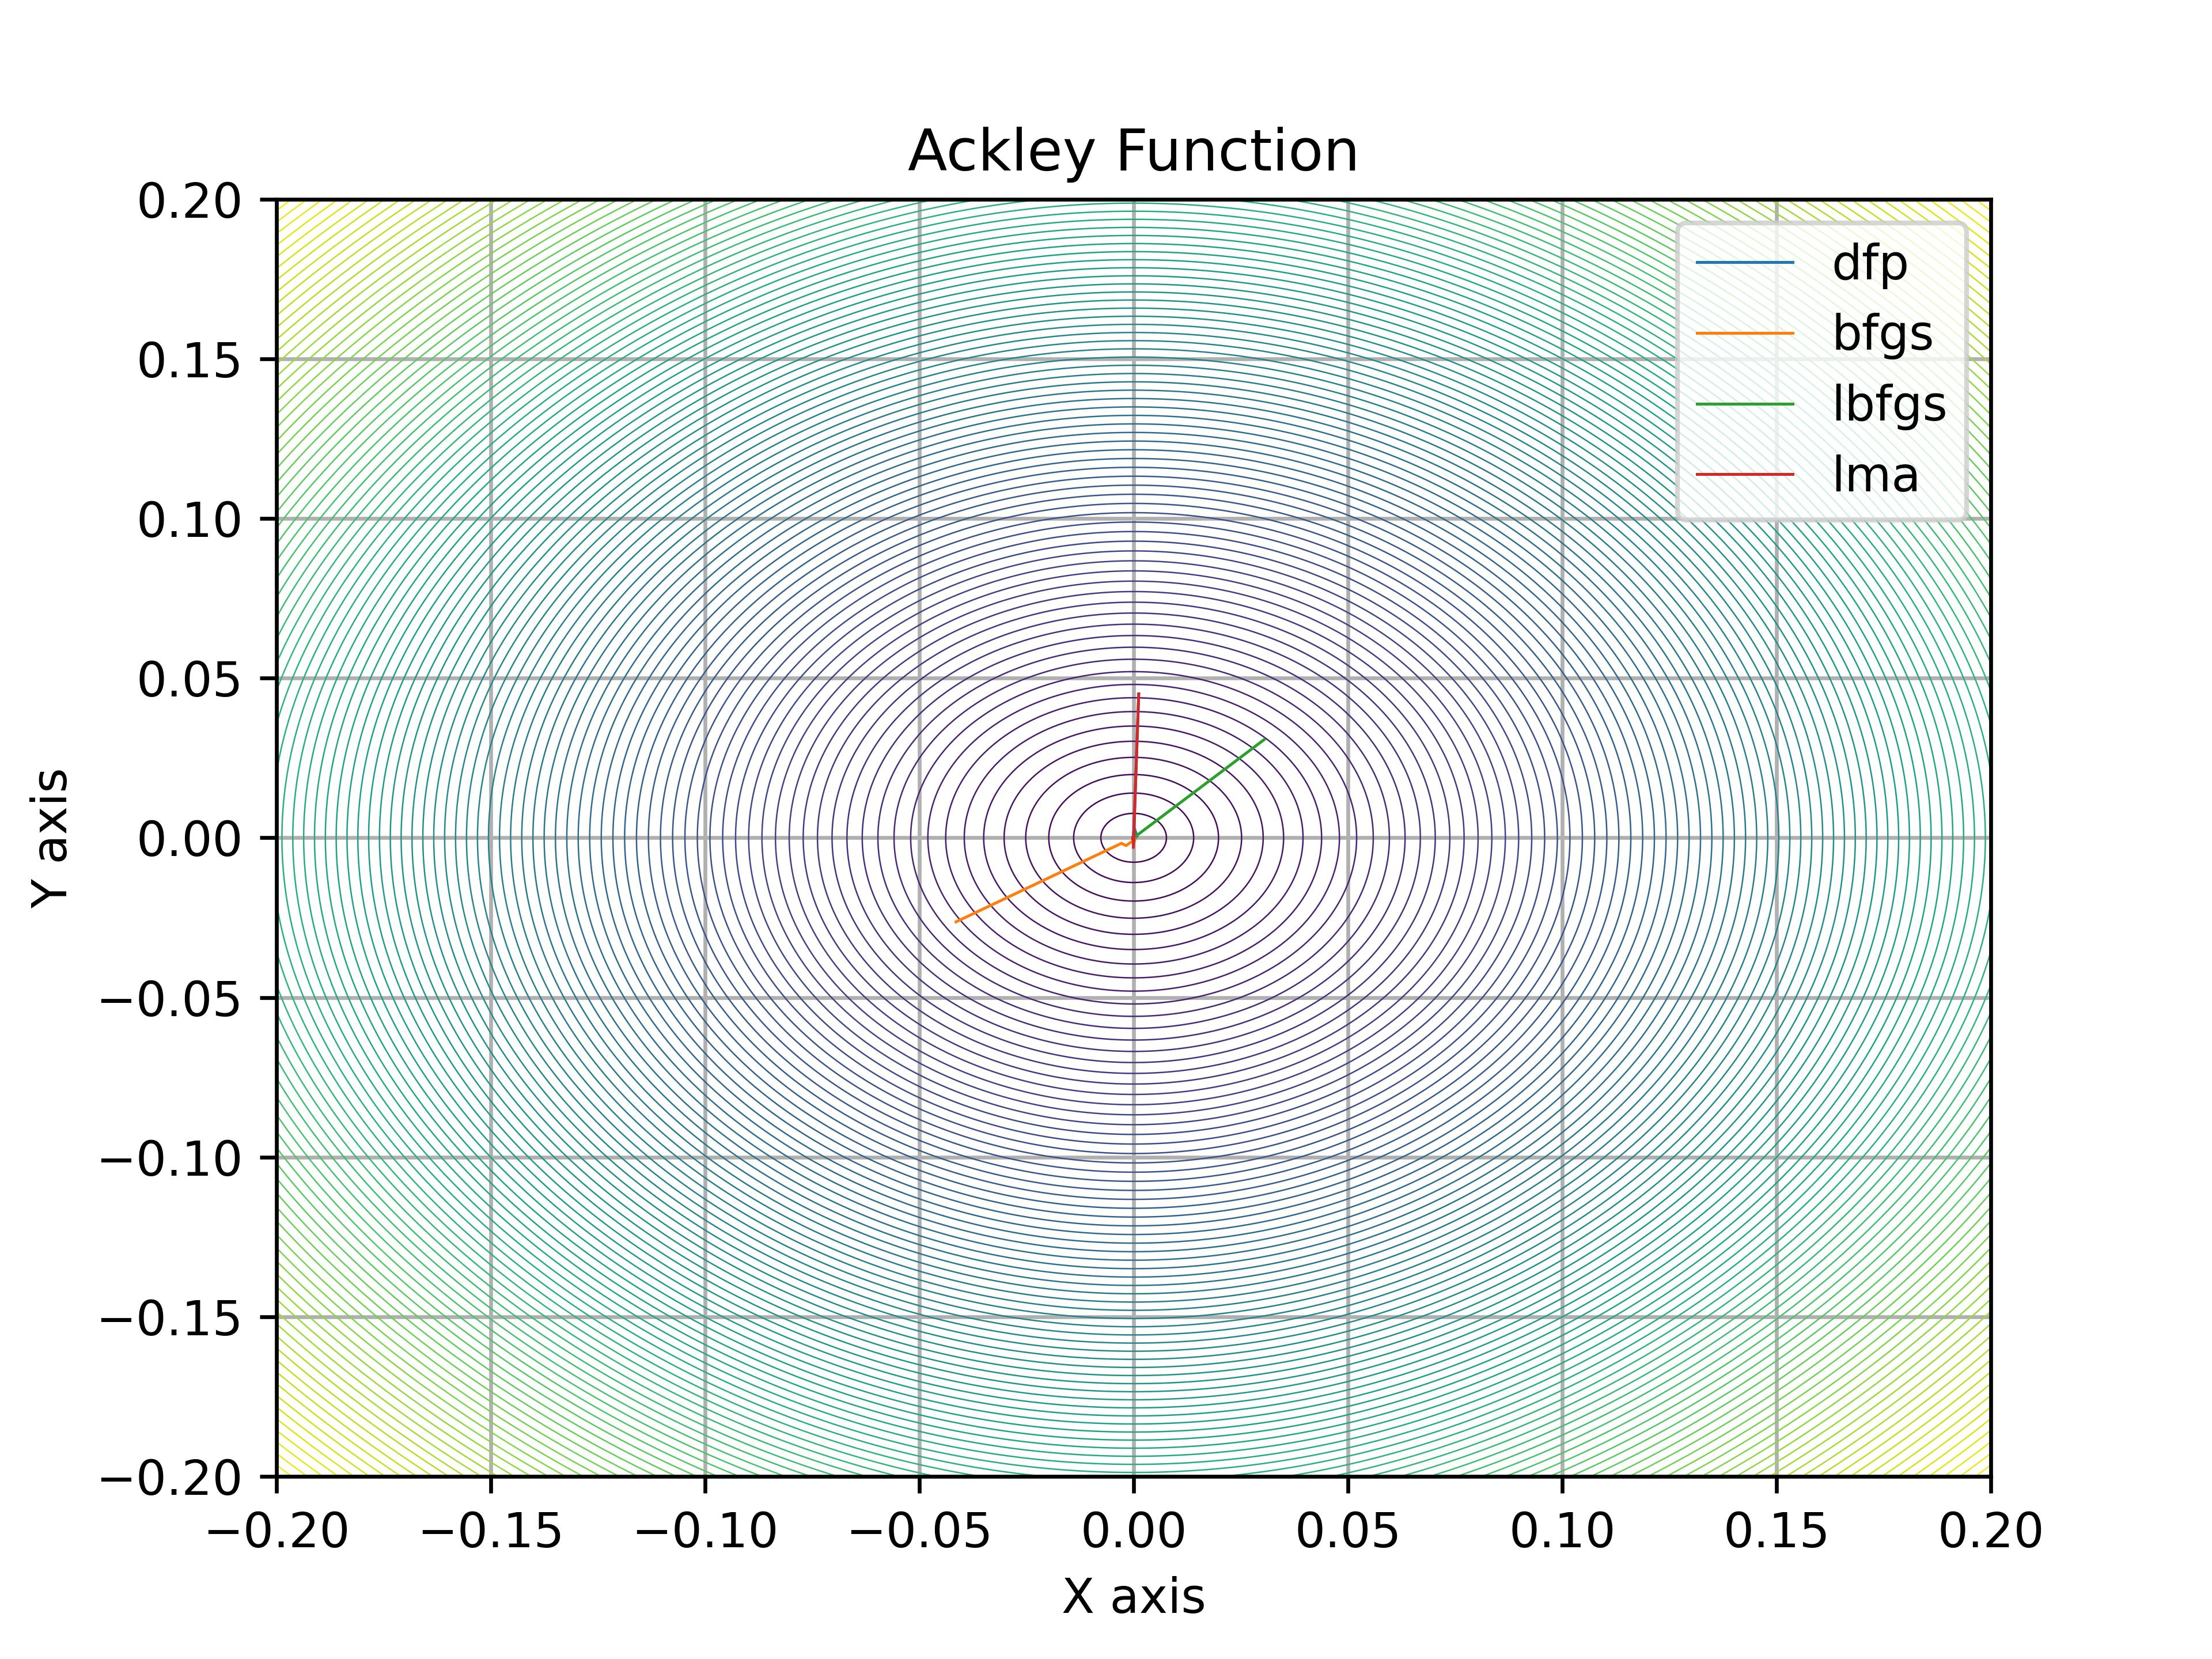
\includegraphics[scale=0.5]{images/ackley.jpg}
\end{figure}
The isolines for Ackley Function shows that there are at least 4 pitfalls near the optimal solution, so, the search space needs to be reduced to $[-0.05, 0.05]$ to avoid wrong convergence. All the algorithms converges quite smoothly following a straight line\subsection{Beale Function}
\label{beale2D}

\subsubsection{Convergence Analysis}
\label{convergencebeale2D}


The convergence report for the Beale Function is shown in Table~\ref{convergence:beale}:

\begin{table}[H]
\centering
\caption{Convergence Report For Beale Function}
\label{convergence:beale}
\begin{tabular}{lrrrr}
\toprule
 Alg. &  Good &  Poor &  Diver. &  Total \\
\midrule
  dfp &    53 &    25 &      22 &    100 \\
 bfgs &    75 &     0 &      25 &    100 \\
lbfgs &    80 &     0 &      20 &    100 \\
  lma &    42 &    37 &      21 &    100 \\
\bottomrule
\end{tabular}
\end{table}

The Table~\ref{convergence:beale} show that not any algorithm
is capable to solve any problem. LMA had the worst performance
in good convergence, followed by DFP, BGFS and LBGFS. LBFGS has
a performance of 80\% in convergence.

The Beale Function seems to have a plateau near the solution, as
it is shown in Section~\ref{isolinesbeale2D}.

\subsubsection{Statistical Analysis of The Solutions}
\label{statisticalanalysisbeale2D}


The minimal. maximal, mean and median values of the solutions are shown in Table~\ref{function_values:beale}:

\begin{table}[H]
\centering
\caption{Statistical Information about function values For Beale Function}
\label{function_values:beale}
\begin{tabular}{lrrrr}
\toprule
 Alg. &  Min &   Max &  Mean &  Median \\
\midrule
  dfp & 0.00 &  3.84 &  0.27 &    0.00 \\
 bfgs & 0.00 &  0.45 &  0.11 &    0.00 \\
lbfgs & 0.00 &  7.31 &  0.36 &    0.00 \\
  lma & 0.00 & 14.20 &  5.35 &    0.45 \\
\bottomrule
\end{tabular}
\end{table}

LMA again had the worst performance. It is the only algorithm that, although has some solutions in
poor convergence, that has a median greater than zero. LBFGS and DFP seems quite radical in terms
of convergence, while having a median of zero its mean values are greater than zero an its maximal
value are noticeable. The larger mean value of LMA reinforces the notion of divergence in this case
and signifies that the algorithm don't fit very well for the Beale Function minimum.


\subsubsection{Best Fits}
\label{bestfitsbeale2D}


The best solutions of all algorithms for Beale Function, obtained using the minimal
distance of the solution, are shown in Table~\ref{solutions:beale}:

\begin{table}[H]
\centering
\caption{Best Fits For Beale Function}
\label{solutions:beale}
\begin{tabular}{llrrr}
\toprule
 Alg. &    Sol. &  Iter. &  F. Eval &  F. Value \\
\midrule
  dfp & $S_{1}$ &      8 &       10 &      0.00 \\
 bfgs & $S_{2}$ &     15 &       18 &      0.00 \\
lbfgs & $S_{3}$ &     14 &       50 &      0.00 \\
  lma & $S_{4}$ &     12 &       13 &      0.00 \\
\bottomrule
\end{tabular}
\end{table}

The Beale function has a very large search space around the optimal solution and
it had a reasonable number of iterations for each algorithm. The DFP method, superseeded by BFGS,
is surprisingly fast to find the solution. The LMA, known to be fast, had a reasonable performance.
BFGS/LBFGS performed as expected.

Although the column F. Value points to the the same value, this is a rounded value
and the real values are of order $10^{-22} \approx 10^{-14}$.



The best solutions of all algorithms for Beale Function, indicated as
$S_{1}$, $S_{2}$, $S_{3}$ and $S_{4}$ in Table~\ref{solutions:beale}, are shown
in Table~\ref{detailedsolutions:beale}:

\begin{table}[H]
\centering
\caption{Detailed Solutions For Beale Function}
\label{detailedsolutions:beale}
\begin{tabular}{lrrrr}
\toprule
 Coord. &  $S_{1}$ &  $S_{2}$ &  $S_{3}$ &  $S_{4}$ \\
\midrule
$x_{1}$ &     3.00 &     3.00 &     3.00 &     3.00 \\
$x_{2}$ &     0.50 &     0.50 &     0.50 &     0.50 \\
\bottomrule
\end{tabular}
\end{table}

The optimal solution for Beale Function is $\left[3, 0.5\right]$ and the rounded values
of Table~\ref{detailedsolutions:beale} points to the same value. The error of
these values are of order $10^{-13}$ os less.



\subsubsection{Isolines and Convergence line}
\label{isolinesbeale2D}

The isolines of Beale Function and convergence lines for all algorithms are shown i Figure~\ref{fig:beale}:\begin{figure}[H]
\centering
\caption{Isolines and convergence line for Beale Function}
\label{fig:beale}
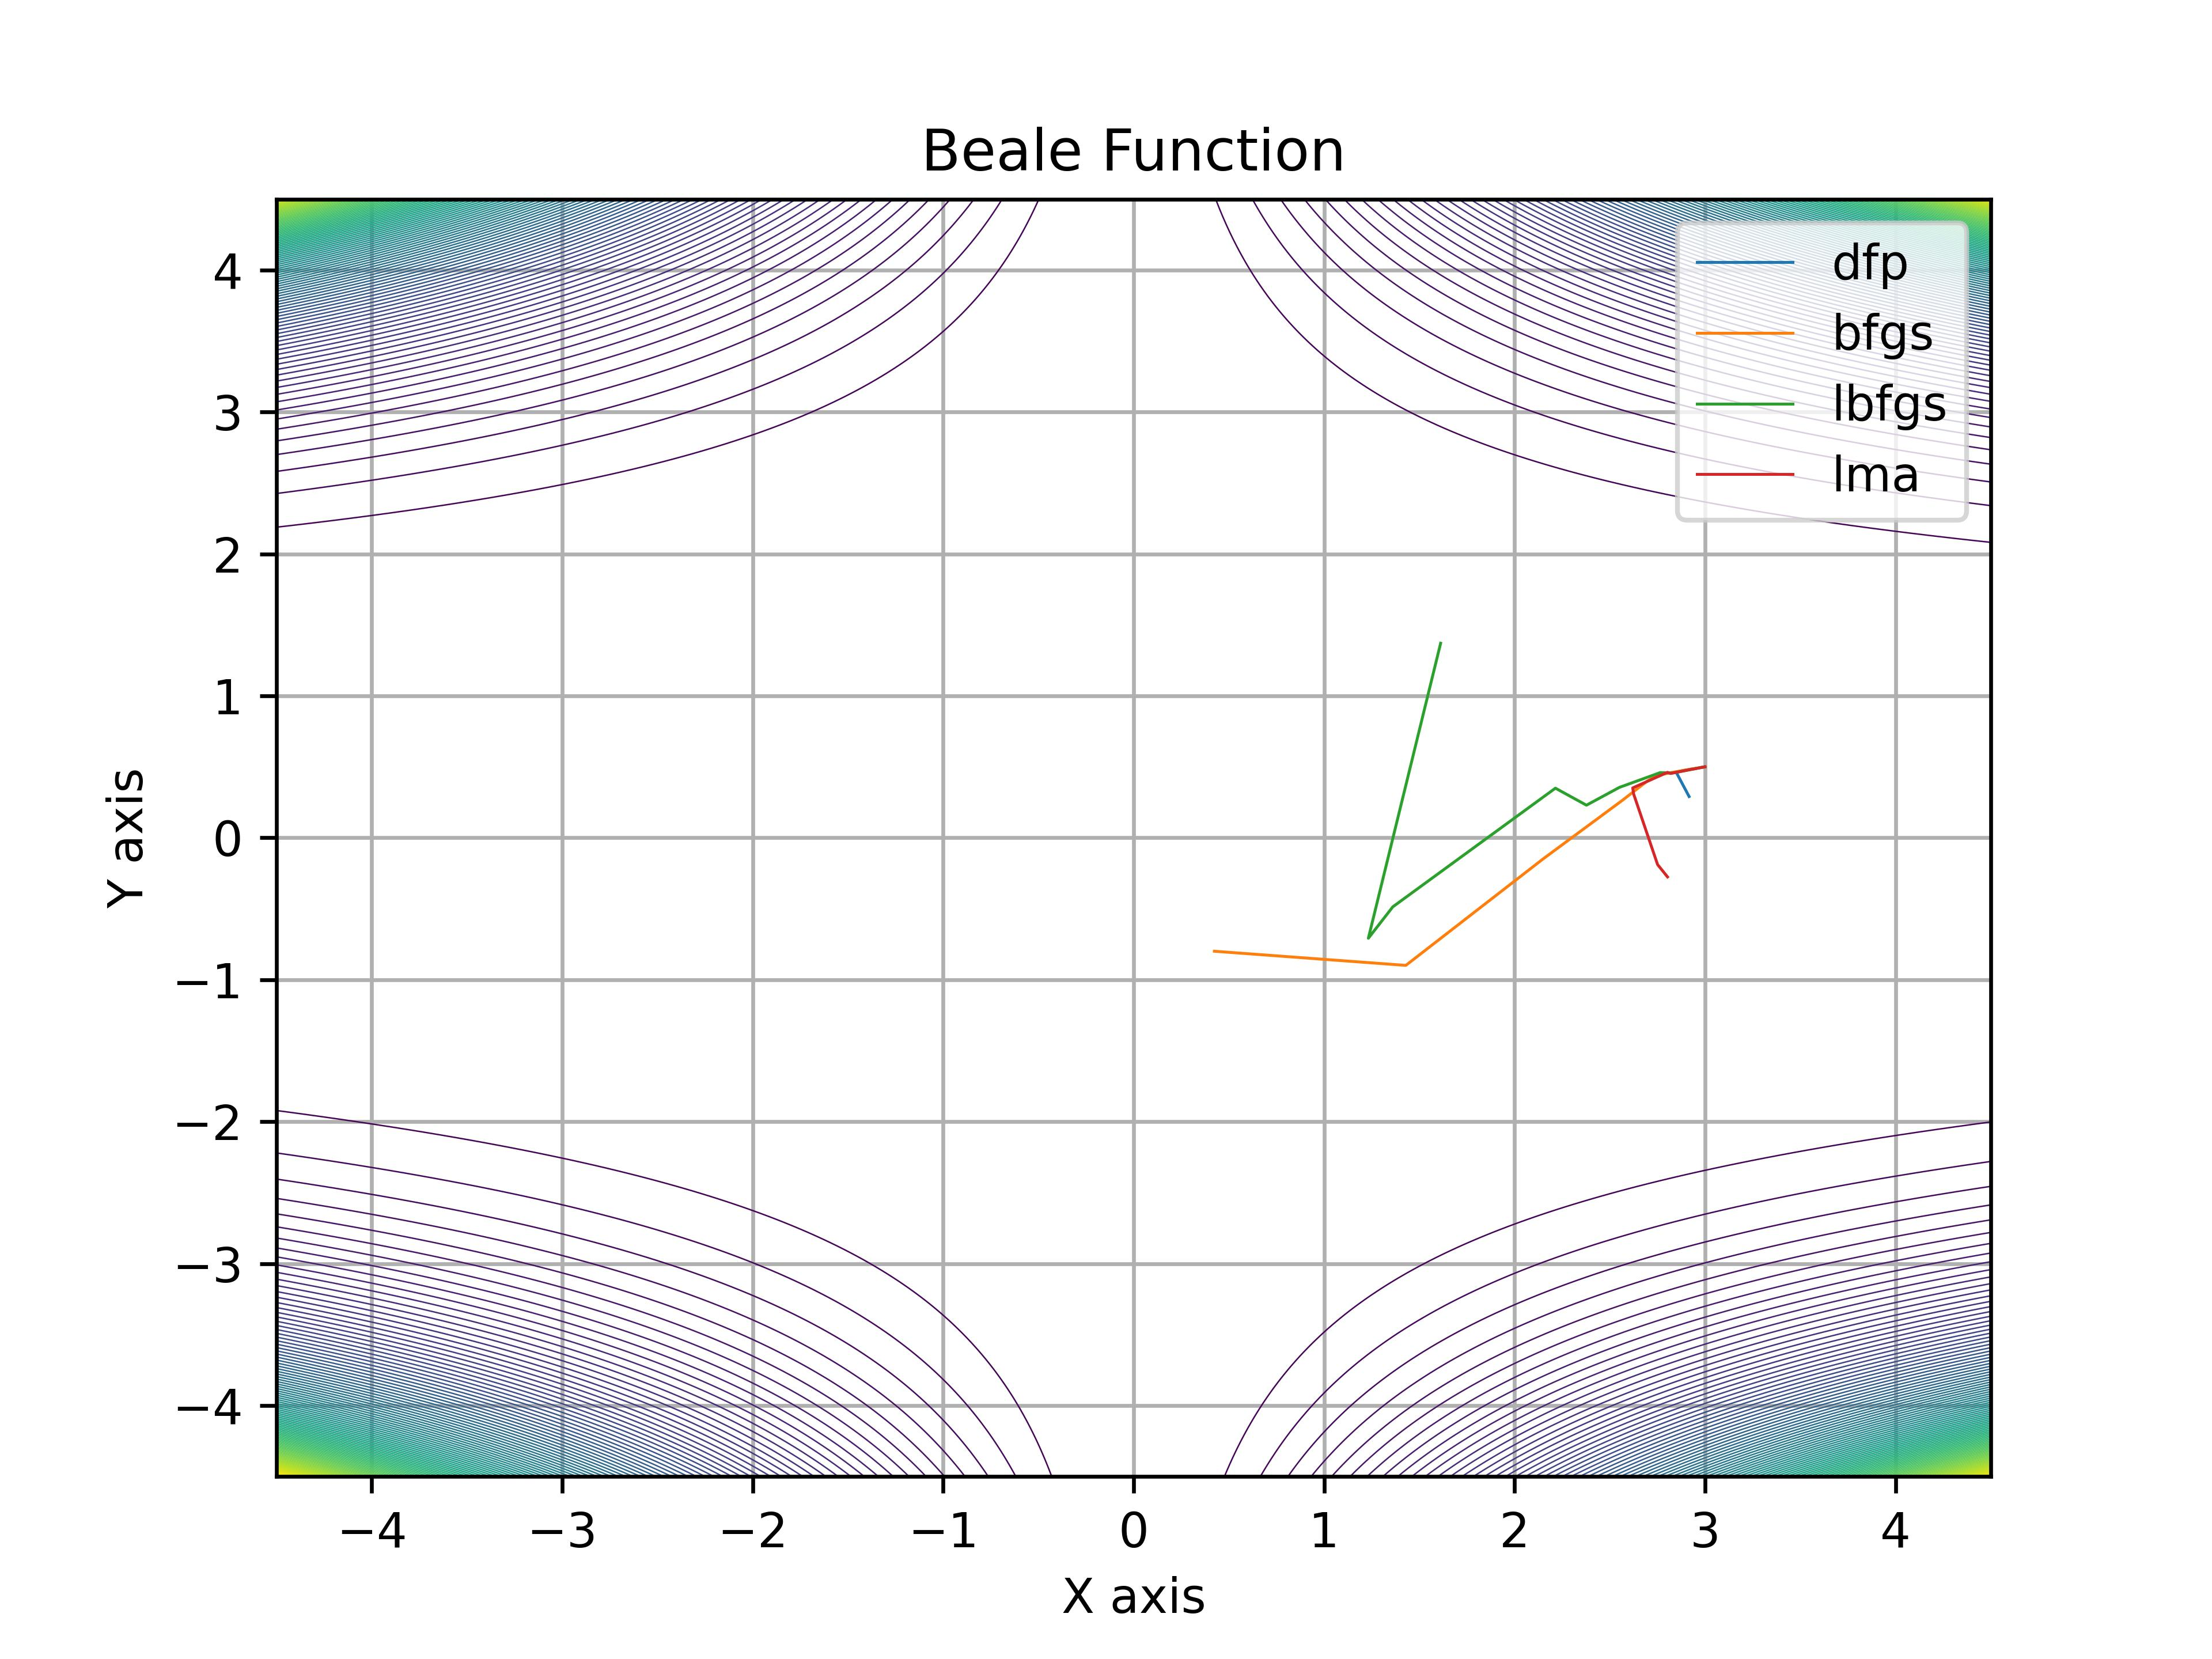
\includegraphics[scale=0.5]{images/beale.jpg}
\end{figure}
The isolines for Beale Function shows that there are a large plateau near the solution. For this reason we believe that the best algorithm had 80\% of performance at its best. Quasi-Newton algorithms suffers to converge when the gradient is less significant.\subsection{Booth Function}
\label{booth2D}

\subsubsection{Convergence Analysis}
\label{convergencebooth2D}


The convergence report for the Booth Function is shown in Table~\ref{convergence:booth}:

\begin{table}[H]
\centering
\caption{Convergence Report For Booth Function}
\label{convergence:booth}
\begin{tabular}{lrrrr}
\toprule
 Alg. &  Good &  Poor &  Diver. &  Total \\
\midrule
  dfp &   100 &     0 &       0 &    100 \\
 bfgs &   100 &     0 &       0 &    100 \\
lbfgs &   100 &     0 &       0 &    100 \\
  lma &   100 &     0 &       0 &    100 \\
\bottomrule
\end{tabular}
\end{table}

All algorithms converged 100 times, using 100 different initial solutions,
for a constrained search space of $\left[0, 4\right]$ . This search space is around
the optimal solution to avoid wrong convergence to a local minimum. In this search space,
Booth Function has a well defined valley that has the solution as its center, as it is shown
in Section~\ref{isolinesbooth2D}.

\subsubsection{Statistical Analysis of The Solutions}
\label{statisticalanalysisbooth2D}


The minimal. maximal, mean and median values of the solutions are shown in Table~\ref{function_values:beale}:

\begin{table}[H]
\centering
\caption{Statistical Information about function values For Booth Function}
\label{function_values:booth}
\begin{tabular}{lrrrr}
\toprule
 Alg. &  Min &  Max &  Mean &  Median \\
\midrule
  dfp & 0.00 & 0.00 &  0.00 &    0.00 \\
 bfgs & 0.00 & 0.00 &  0.00 &    0.00 \\
lbfgs & 0.00 & 0.00 &  0.00 &    0.00 \\
  lma & 0.00 & 0.00 &  0.00 &    0.00 \\
\bottomrule
\end{tabular}
\end{table}

The values again are rounded. The median informs us that, for all
algorithms is expected to find the minimun of Booth Function.

\subsubsection{Best Fits}
\label{bestfitsbooth2D}


The best solutions of all algorithms for Booth Function, obtained using the minimal
distance of the solution, are shown in Table~\ref{solutions:booth}:

\begin{table}[H]
\centering
\caption{Best Fits For Booth Function}
\label{solutions:booth}
\begin{tabular}{llrrr}
\toprule
 Alg. &    Sol. &  Iter. &  F. Eval &  F. Value \\
\midrule
  dfp & $S_{1}$ &      4 &        6 &      0.00 \\
 bfgs & $S_{2}$ &      2 &        5 &      0.00 \\
lbfgs & $S_{3}$ &      5 &       21 &      0.00 \\
  lma & $S_{4}$ &     10 &       11 &      0.00 \\
\bottomrule
\end{tabular}
\end{table}


Although the column F. Value points to the the same value, this is a rounded value
and the real values are os order $10^{-22} \approx 10^{-14}$.


The best solutions of all algorithms for Beale Function, indicated as
$S_{1}$, $S_{2}$, $S_{3}$ and $S_{4}$ in Table~\ref{solutions:booth}, are shown
in Table~\ref{detailedsolutions:booth}:

\begin{table}[H]
\centering
\caption{Detailed Solutions For Booth Function}
\label{detailedsolutions:booth}
\begin{tabular}{lrrrr}
\toprule
 Coord. &  $S_{1}$ &  $S_{2}$ &  $S_{3}$ &  $S_{4}$ \\
\midrule
$x_{1}$ &     1.00 &     1.00 &     1.00 &     1.00 \\
$x_{2}$ &     3.00 &     3.00 &     3.00 &     3.00 \\
\bottomrule
\end{tabular}
\end{table}

The optimal solution for Booth Function is $\left[1, 3\right]$ and the rounded values
of Table~\ref{detailedsolutions:booth} points to the same value. The error of
these values are of order $10^{-13}$ os less.
\subsubsection{Isolines and Convergence line}
\label{isolinesbooth2D}

The isolines of Booth Function and convergence lines for all algorithms are shown i Figure~\ref{fig:booth}:\begin{figure}[H]
\centering
\caption{Isolines and convergence line for Booth Function}
\label{fig:booth}
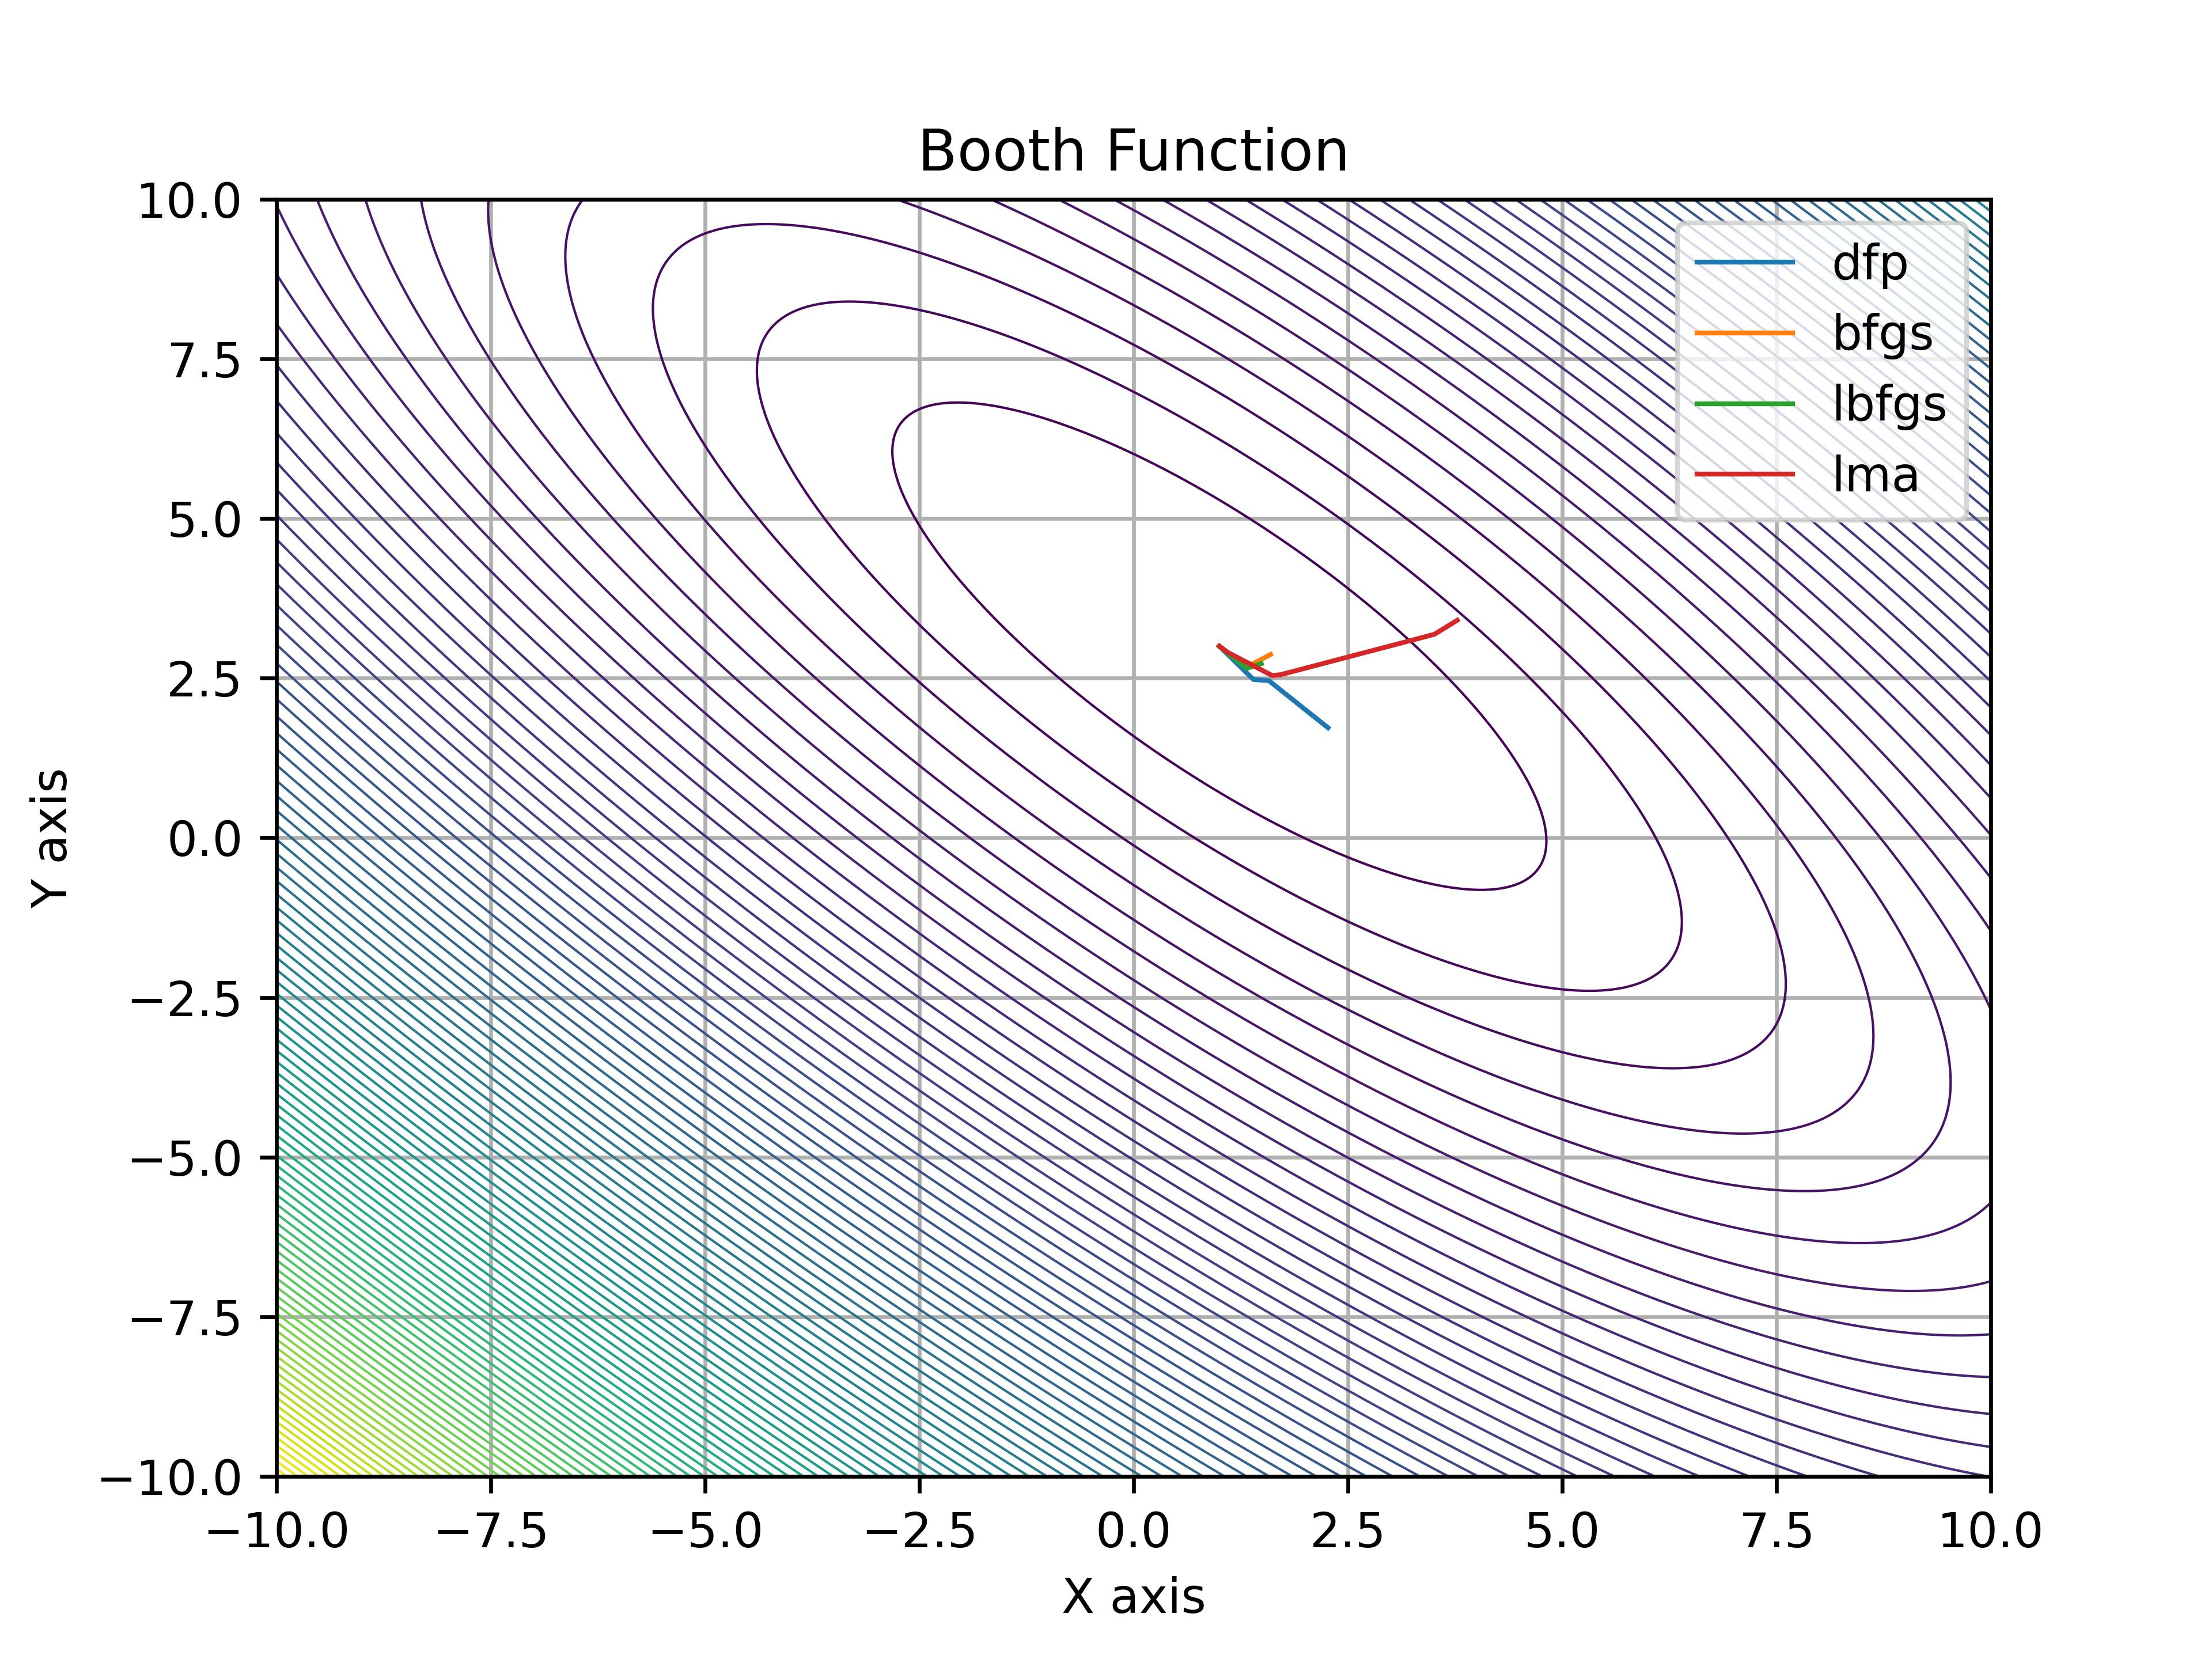
\includegraphics[scale=0.5]{images/booth.jpg}
\end{figure}
The Figure~\ref{fig:booth} shows that Booth Function has a well defined valley near $[1, 3]$. \subsection{Matyas Function}
\label{matyas2D}

\subsubsection{Convergence Analysis}
\label{convergencematyas2D}


The convergence report for the Matyas Function is shown in Table~\ref{convergence:matyas}:

\begin{table}[H]
\centering
\caption{Convergence Report For Matyas Function}
\label{convergence:matyas}
\begin{tabular}{lrrrr}
\toprule
 Alg. &  Good &  Poor &  Diver. &  Total \\
\midrule
  dfp &   100 &     0 &       0 &    100 \\
 bfgs &   100 &     0 &       0 &    100 \\
lbfgs &   100 &     0 &       0 &    100 \\
  lma &   100 &     0 &       0 &    100 \\
\bottomrule
\end{tabular}
\end{table}

All algorithms converged 100 times, using 100 different initial solutions,
for a search space of $\left[-10, 10\right]$ . In this search space,
Matyas Function has a well defined valley that has the solution as its
center, as it is shown in Section~\ref{isolinesmatyas2D}.

\subsubsection{Statistical Analysis of The Solutions}
\label{statisticalanalysismatyas2D}


The minimal. maximal, mean and median values of the solutions are shown in Table~\ref{function_values:matyas}:

\begin{table}[H]
\centering
\caption{Statistical Information about function values For Matyas Function}
\label{function_values:matyas}
\begin{tabular}{lrrrr}
\toprule
 Alg. &  Min &  Max &  Mean &  Median \\
\midrule
  dfp & 0.00 & 0.00 &  0.00 &    0.00 \\
 bfgs & 0.00 & 0.00 &  0.00 &    0.00 \\
lbfgs & 0.00 & 0.00 &  0.00 &    0.00 \\
  lma & 0.00 & 0.00 &  0.00 &    0.00 \\
\bottomrule
\end{tabular}
\end{table}

The values again are rounded. The median informs us that, for all
algorithms is expected to find the minimun of Matyas Function.
\subsubsection{Best Fits}
\label{bestfitsmatyas2D}


The best solutions of all algorithms for Booth Function, obtained using the minimal
distance of the solution, are shown in Table~\ref{solutions:matyas}:

\begin{table}[H]
\centering
\caption{Best Fits For Matyas Function}
\label{solutions:matyas}
\begin{tabular}{llrrr}
\toprule
 Alg. &    Sol. &  Iter. &  F. Eval &  F. Value \\
\midrule
  dfp & $S_{1}$ &      7 &       10 &      0.00 \\
 bfgs & $S_{2}$ &      7 &       10 &      0.00 \\
lbfgs & $S_{3}$ &      4 &       16 &      0.00 \\
  lma & $S_{4}$ &     14 &       15 &      0.00 \\
\bottomrule
\end{tabular}
\end{table}

The algorithms DFP, BFGS and LBFGS have comparable performances, while LMA
is the most expensive of all.

Although the column F. Value points to the the same value, this is a rounded value
and the real values are os order $10^{-22} \approx 10^{-14}$.



The best solutions of all algorithms for Matyas Function, indicated as
$S_{1}$, $S_{2}$, $S_{3}$ and $S_{4}$ in Table~\ref{solutions:matyas}, are shown
in Table~\ref{detailedsolutions:matyas}:

\begin{table}[H]
\centering
\caption{Detailed Solutions For Matyas Function}
\label{detailedsolutions:matyas}
\begin{tabular}{lrrrr}
\toprule
 Coord. &  $S_{1}$ &  $S_{2}$ &  $S_{3}$ &  $S_{4}$ \\
\midrule
$x_{1}$ &     0.00 &    -0.00 &    -0.00 &     0.00 \\
$x_{2}$ &     0.00 &    -0.00 &     0.00 &     0.00 \\
\bottomrule
\end{tabular}
\end{table}

The optimal solution for Matyas Function is $\left[0, 0\right]$ and the rounded values
of Table~\ref{detailedsolutions:matyas} points to the same value. The error of
these values are of order $10^{-13}$ os less.
\subsubsection{Isolines and Convergence line}
\label{isolinesmatyas2D}

The isolines of Matyas Function and convergence lines for all algorithms are shown i Figure~\ref{fig:matyas}:\begin{figure}[H]
\centering
\caption{Isolines and convergence line for Matyas Function}
\label{fig:matyas}
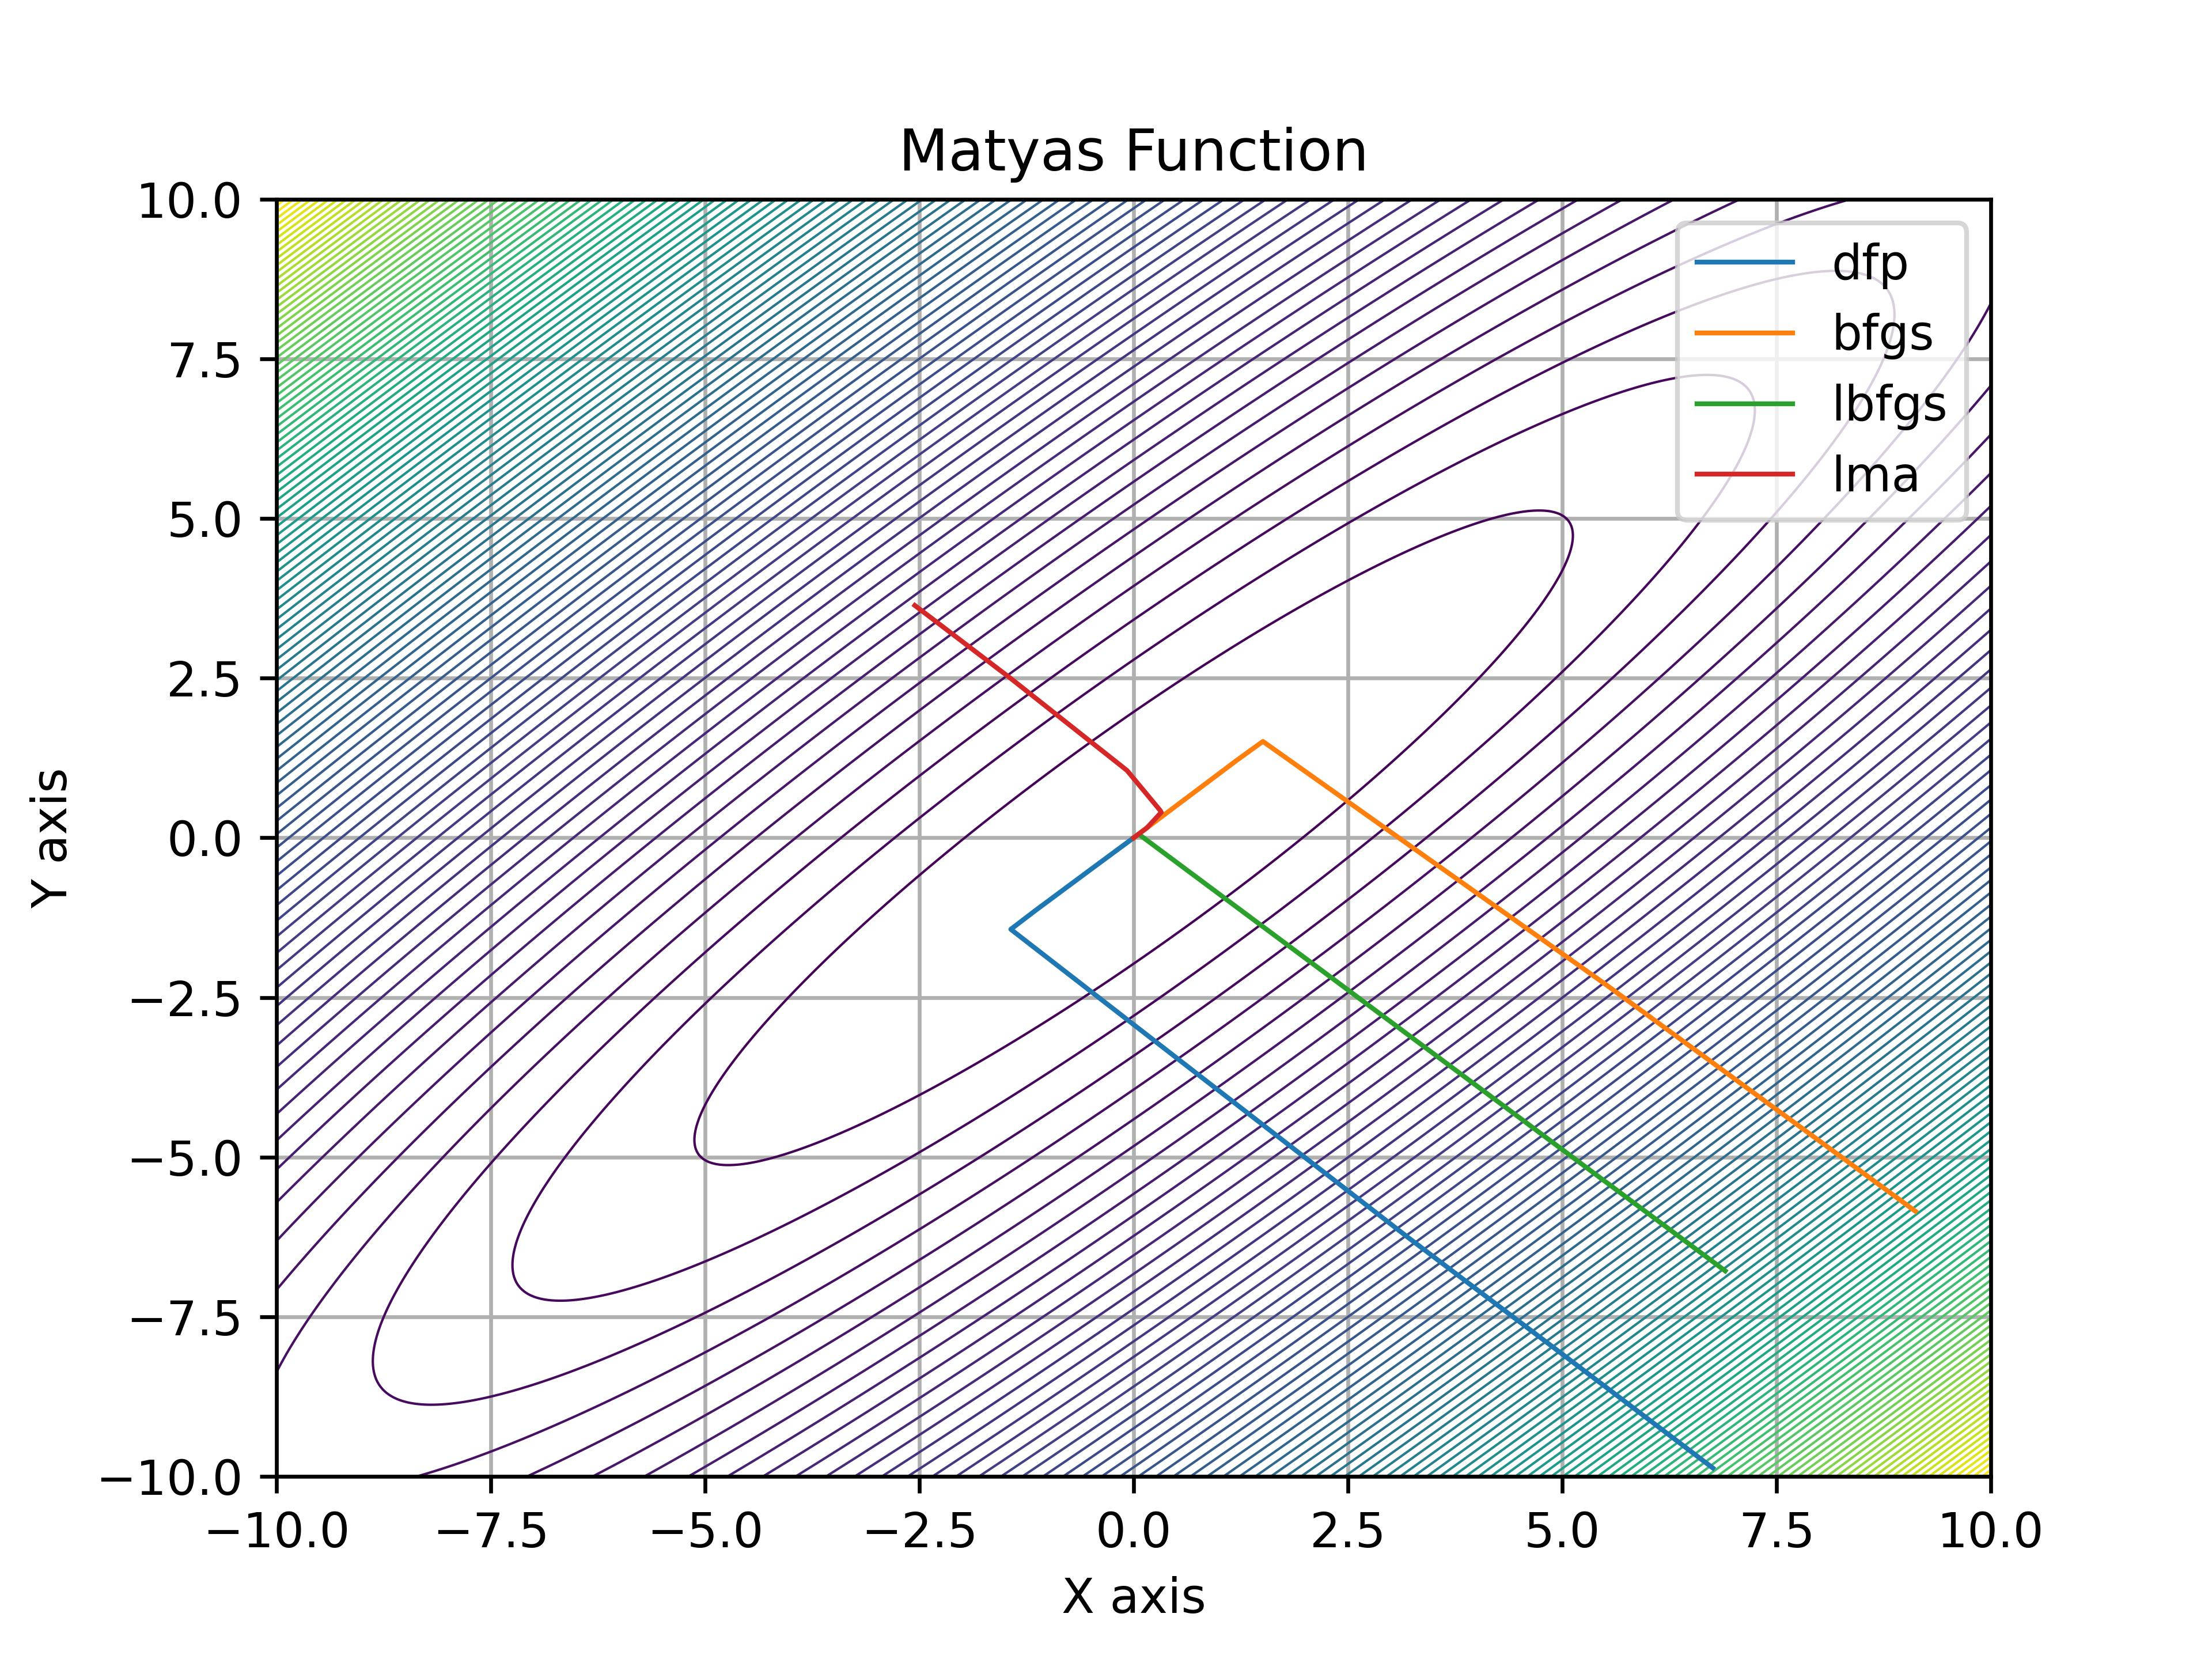
\includegraphics[scale=0.5]{images/matyas.jpg}
\end{figure}
The Figure~\ref{fig:matyas} shows that Matyas Function has a well defined valley near $[0, 0]$. \subsection{Rastrigin Function}
\label{rastrigin2d2D}

\subsubsection{Convergence Analysis}
\label{convergencerastrigin2d2D}


The convergence report for the Rastrigin Function in 2 dimensions is shown in Table~\ref{convergence:rastrigin2d}:

\begin{table}[H]
\centering
\caption{Convergence Report For Rastrigin Function}
\label{convergence:rastrigin2d}
\begin{tabular}{lrrrr}
\toprule
 Alg. &  Good &  Poor &  Diver. &  Total \\
\midrule
  dfp &   100 &     0 &       0 &    100 \\
 bfgs &   100 &     0 &       0 &    100 \\
lbfgs &    99 &     1 &       0 &    100 \\
  lma &   100 &     0 &       0 &    100 \\
\bottomrule
\end{tabular}
\end{table}

It is quite sure that all algorithms has good convergence for any algorithm for a
constrained search space of $\left[-0.15, 0.15\right]$. This search space is around
the optimal solution to avoid wrong convergence to a local minimum. In this search space,
Rastrigin Function has a well defined valley that has the solution as its center, as is shown in
Section~\ref{isolinesrastrigin2D}.

\subsubsection{Statistical Analysis of The Solutions}
\label{statisticalanalysisrastrigin2d2D}


The minimal. maximal, mean and median values of the solutions are shown in Table~\ref{function_values:rastrigin2d}:

\begin{table}[H]
\centering
\caption{Statistical Information about function values For Rastrigin Function}
\label{function_values:rastrigin2d}
\begin{tabular}{lrrrr}
\toprule
 Alg. &  Min &  Max &  Mean &  Median \\
\midrule
  dfp & 0.00 & 0.00 &  0.00 &    0.00 \\
 bfgs & 0.00 & 0.00 &  0.00 &    0.00 \\
lbfgs & 0.00 & 1.99 &  0.02 &    0.00 \\
  lma & 0.00 & 0.00 &  0.00 &    0.00 \\
\bottomrule
\end{tabular}
\end{table}

The values again are rounded. The median informs us that, for all
algorithms is expected to find the minimun of Rastrigin Function.
Although the mean of LBFGS algorithm is greater than zero, it is expected
to converge mora than diverge in the function constrained search space.
\subsubsection{Best Fits}
\label{bestfitsrastrigin2d2D}


The best solutions of all algorithms for Rastrigin Function, obtained using the minimal
distance of the solution, are shown in Table~\ref{solutions:rastrigin2d}:

\begin{table}[H]
\centering
\caption{Best Fits For Rastrigin Function}
\label{solutions:rastrigin2d}
\begin{tabular}{llrrr}
\toprule
 Alg. &    Sol. &  Iter. &  F. Eval &  F. Value \\
\midrule
  dfp & $S_{1}$ &      6 &       11 &      0.00 \\
 bfgs & $S_{2}$ &      8 &       49 &      0.00 \\
lbfgs & $S_{3}$ &      5 &      133 &      0.00 \\
  lma & $S_{4}$ &      4 &        5 &      0.00 \\
\bottomrule
\end{tabular}
\end{table}

LMA is the less expensive algorithm to solve Rastrigin in 2 dimensions, while LBFGS
is the most expensive of all. Although it has one more iteration than LMA, it evaluates
the objective function much more times than BFGS, the second most expensive algorithm.

Although the column F. Value points to the the same value, this is a rounded value
and the real values are os order $10^{-22} \approx 10^{-14}$.

The best solutions of all algorithms for Rastrigin Function, indicated as
$S_{1}$, $S_{2}$, $S_{3}$ and $S_{4}$ in Table~\ref{solutions:rastrigin2d}, are shown
in Table~\ref{detailedsolutions:rastrigin2d}:

\begin{table}[H]
\centering
\caption{Detailed Solutions For Rastrigin Function}
\label{detailedsolutions:rastrigin2d}
\begin{tabular}{lrrrr}
\toprule
 Coord. &  $S_{1}$ &  $S_{2}$ &  $S_{3}$ &  $S_{4}$ \\
\midrule
$x_{1}$ &    -0.00 &     0.00 &     0.00 &     0.00 \\
$x_{2}$ &     0.00 &    -0.00 &    -0.00 &     0.00 \\
\bottomrule
\end{tabular}
\end{table}

The Table~\ref{detailedsolutions:rastrigin2d} shows the same solution to all algorithms, because the values are so small
and were rounded to fit on the Table. The differences of the optimal point are of order $10^{-14}$ to $10^{-22}$,
for the LMA, DFP, LBFGS and BFGS algorithms, respectively.

\subsubsection{Isolines and Convergence line}
\label{isolinesrastrigin2d2D}

The isolines of Rastrigin Function for 2 dimensions and convergence lines for all algorithms are shown in Figure~\ref{fig:rastrigin2d}:\begin{figure}[H]
\centering
\caption{Isolines and convergence line for Rastrigin Function}
\label{fig:rastrigin2d}
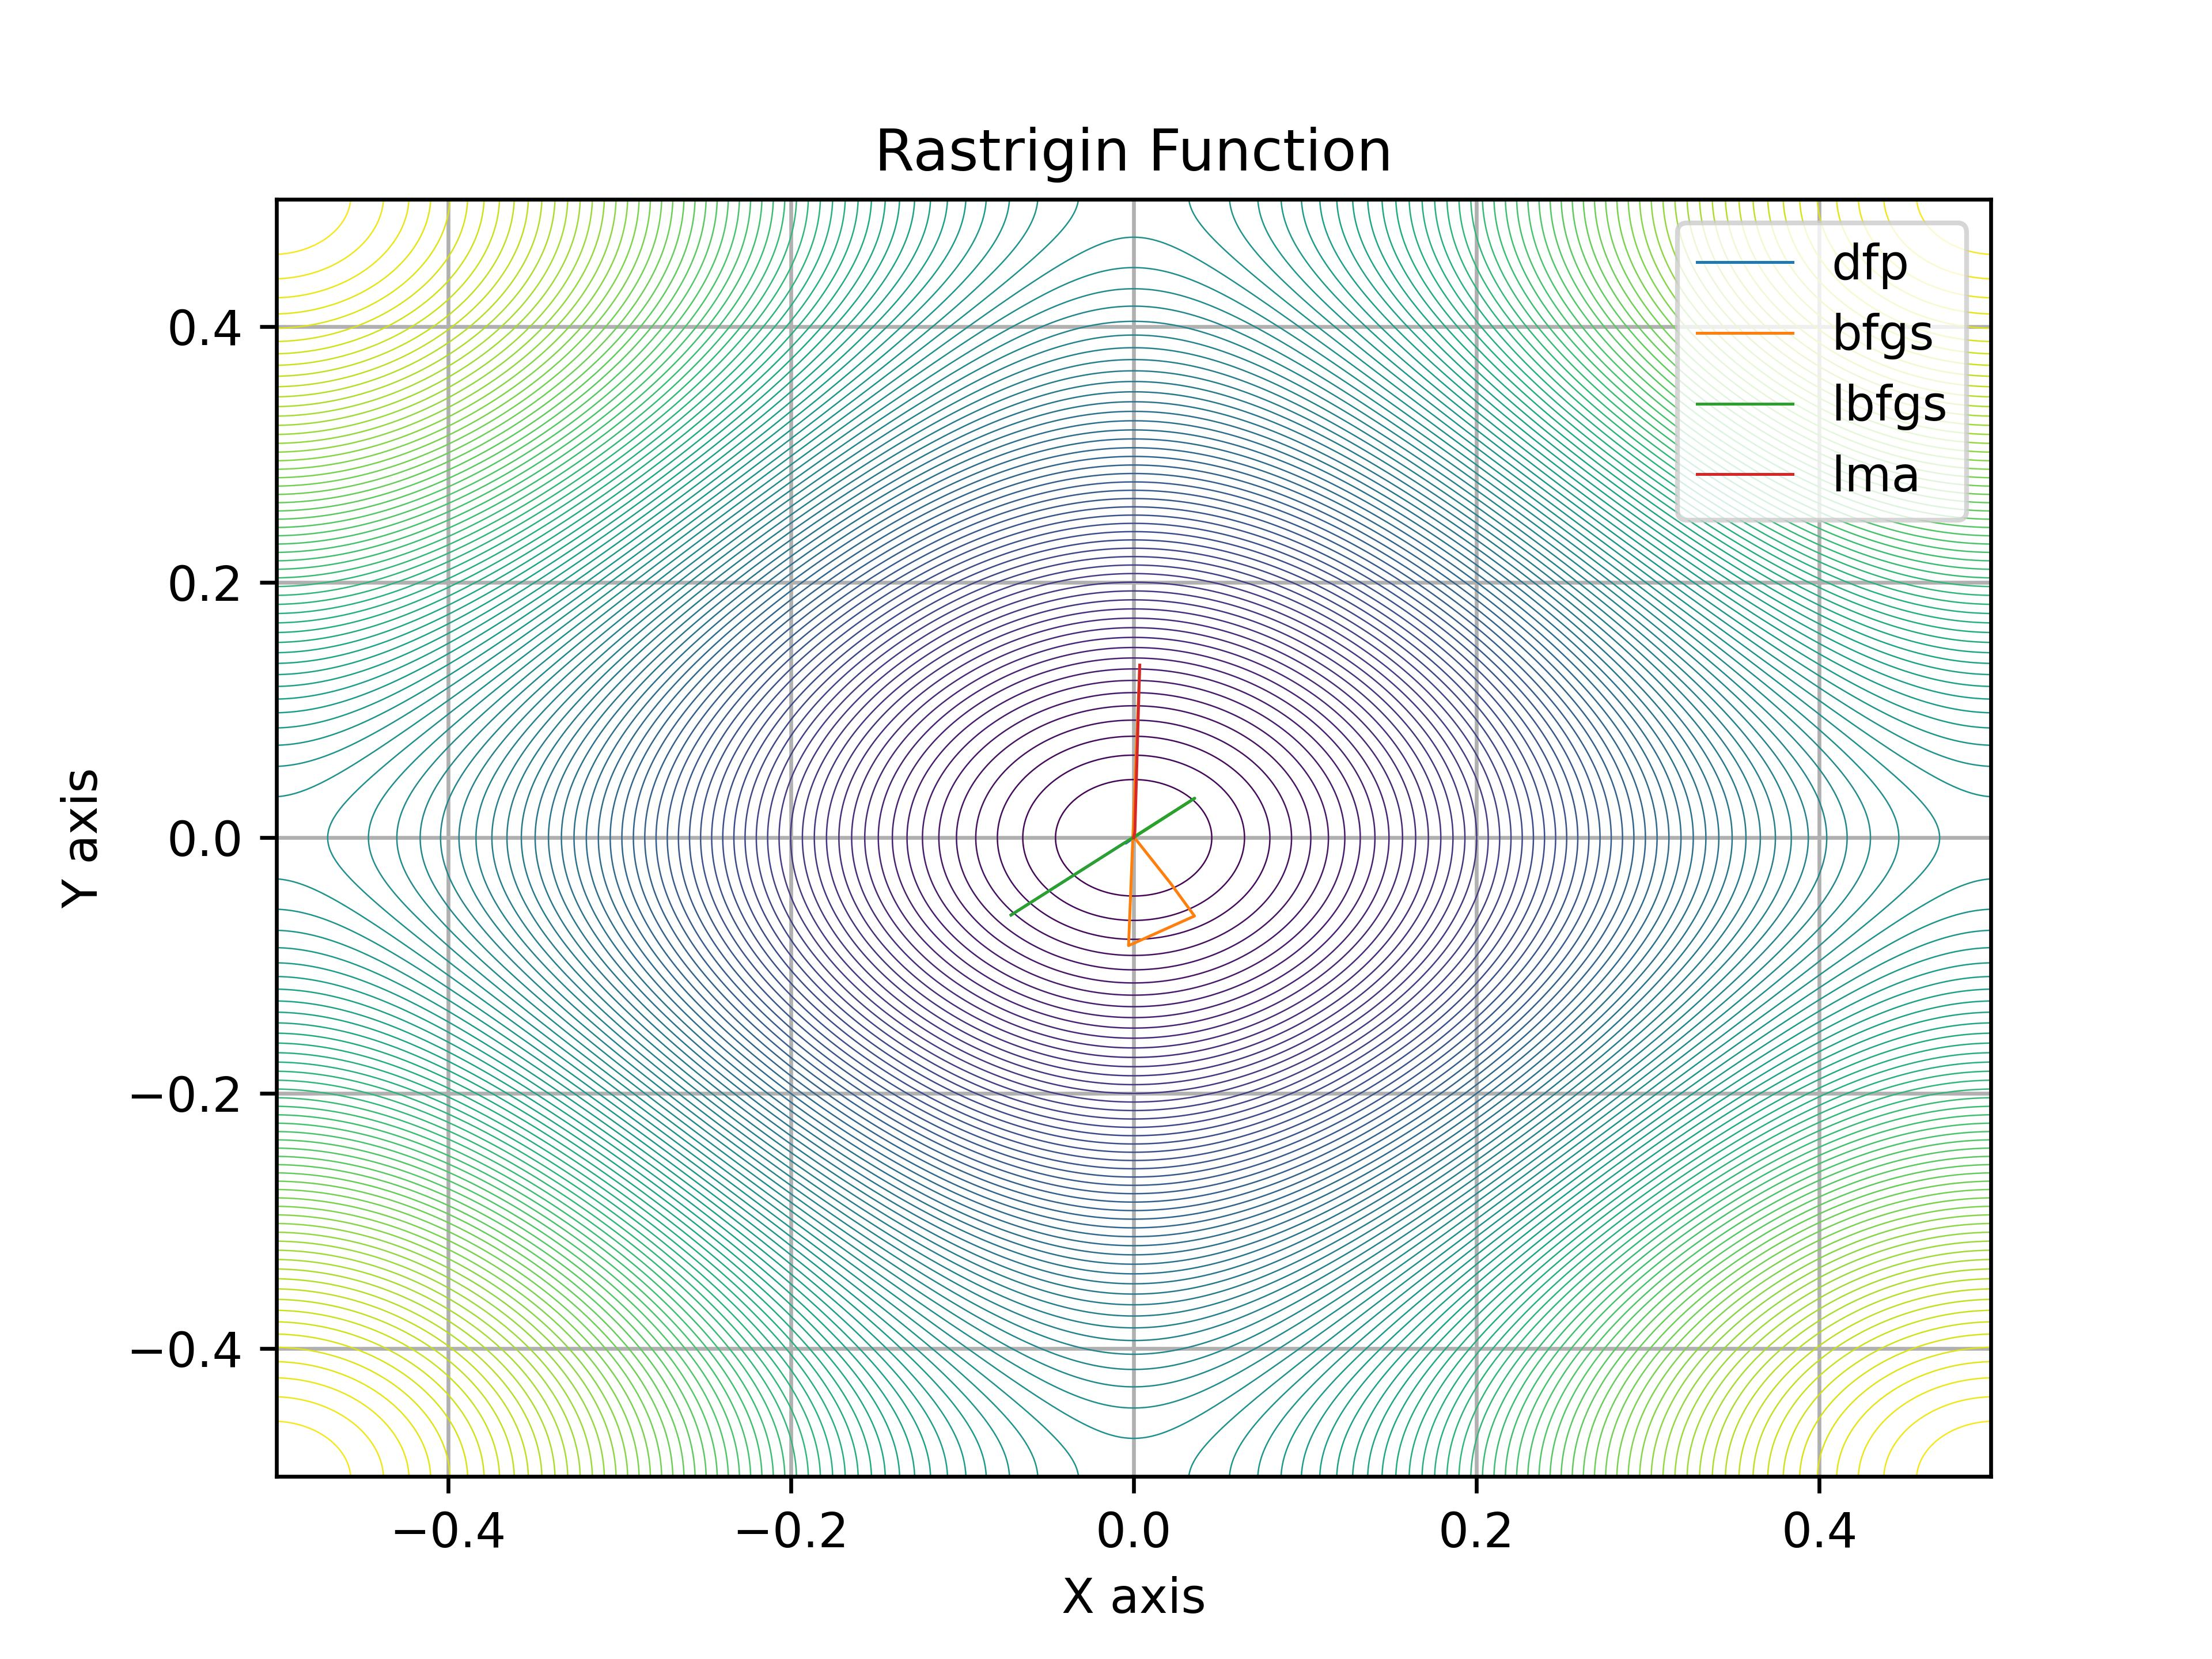
\includegraphics[scale=0.5]{images/rastrigin2d.jpg}
\end{figure}
The isolines for Rastrigin Function shows that there are at least 2 pitfalls near the optimal solution, so, the search space needs to be reduced to $[-0.15, 0.15]$ to avoid wrong convergence. All the algorithms, except BFGS, converges quite smoothly following a straight line\subsection{Rosenbrock Function}
\label{rosenbrock2d2D}

\subsubsection{Convergence Analysis}
\label{convergencerosenbrock2d2D}


The convergence report for the Rosenbrock Function in 30 dimensions is shown in Table~\ref{convergence:rosenbrock2d}:

\begin{table}[H]
\centering
\caption{Convergence Report For Rosenbrock Function}
\label{convergence:rosenbrock2d}
\begin{tabular}{lrrrr}
\toprule
 Alg. &  Good &  Poor &  Diver. &  Total \\
\midrule
  dfp &    74 &    26 &       0 &    100 \\
 bfgs &   100 &     0 &       0 &    100 \\
lbfgs &   100 &     0 &       0 &    100 \\
  lma &   100 &     0 &       0 &    100 \\
\bottomrule
\end{tabular}
\end{table}

Except for DFP, Rosenbrock has good convergence for any algorithm for a constrained search space
of $\left[-1.5, 1.5\right]$. Although the Rosenbrock Function has only the global minimum in a
search space of $\left[-10, 10\right]$, it has a large banana shaped plateau near the optimal
solution, as it is shown in Section~\ref{isolinesrosenbrock2D}. The search space constraint serves
only to limit the number of iterations of each algorithm. The large search space tends to make the algorithm
walks too much to find the solution and tends to exceed the maximum iterations defined in the evaluation
criteria shown in Section~\ref{sec:introduction}.

\subsubsection{Statistical Analysis of The Solutions}
\label{statisticalanalysisrosenbrock2d2D}


The minimal. maximal, mean and median values of the solutions are shown in Table~\ref{function_values:rosenbrock2d}:

\begin{table}[H]
\centering
\caption{Statistical Information about function values For Rosenbrock Function}
\label{function_values:rosenbrock2d}
\begin{tabular}{lrrrr}
\toprule
 Alg. &  Min &  Max &  Mean &  Median \\
\midrule
  dfp & 0.00 & 1.33 &  0.04 &    0.00 \\
 bfgs & 0.00 & 0.00 &  0.00 &    0.00 \\
lbfgs & 0.00 & 0.00 &  0.00 &    0.00 \\
  lma & 0.00 & 0.00 &  0.00 &    0.00 \\
\bottomrule
\end{tabular}
\end{table}

The values again are rounded. The median informs us that, for all
algorithms is expected to find the minimun of Rosenbrock Function.
Although the mean of DFP algorithm is greater than zero, it is expected
to converge more than diverge in the function constrained search space.
\subsubsection{Best Fits}
\label{bestfitsrosenbrock2d2D}


The best solutions of all algorithms for Rosenbrock Function, obtained using the minimal
distance of the solution, are shown in Table~\ref{solutions:rosenbrock2d}:

\begin{table}[H]
\centering
\caption{Best Fits For Rosenbrock Function}
\label{solutions:rosenbrock2d}
\begin{tabular}{llrrr}
\toprule
 Alg. &    Sol. &  Iter. &  F. Eval &  F. Value \\
\midrule
  dfp & $S_{1}$ &     24 &       31 &      0.00 \\
 bfgs & $S_{2}$ &     30 &       43 &      0.00 \\
lbfgs & $S_{3}$ &     27 &       76 &      0.00 \\
  lma & $S_{4}$ &     16 &       18 &      0.00 \\
\bottomrule
\end{tabular}
\end{table}

LMA is the less expensive algorithm to solve Rosenbrock Function in 2 dimensions, while LBFGS
is the most expensive of all. Although it has comparable iterations with DFP nd BFGS, it evaluates
the objective function twice as much of BFGS, the second most expensive algorithm.

Although the column F. Value points to the the same value, this is a rounded value
and the real values are os order $10^{-22} \approx 10^{-14}$.

The best solutions of all algorithms for Rosenbrock Function, indicated as
$S_{1}$, $S_{2}$, $S_{3}$ and $S_{4}$ in Table~\ref{solutions:rosenbrock2d}, are shown
in Table~\ref{detailedsolutions:rosenbrock2d}:

\begin{table}[H]
\centering
\caption{Detailed Solutions For Rosenbrock Function}
\label{detailedsolutions:rosenbrock2d}
\begin{tabular}{lrrrr}
\toprule
 Coord. &  $S_{1}$ &  $S_{2}$ &  $S_{3}$ &  $S_{4}$ \\
\midrule
$x_{1}$ &     1.00 &     1.00 &     1.00 &     1.00 \\
$x_{2}$ &     1.00 &     1.00 &     1.00 &     1.00 \\
\bottomrule
\end{tabular}
\end{table}

The optimal point of Rosenbrock function in 2 dimensions is correctly pointed to $\left[1, 1\right]$. The Table~\ref{detailedsolutions:rosenbrock2d}
shows the same solution to all algorithms, because the values are so small and were rounded to fit on the Table. The differences of
the optimal point are of order $10^{-14}$ to $10^{-22}$, for the LMA, DFP, LBFGS and BFGS algorithms, respectively.

\subsubsection{Isolines and Convergence line}
\label{isolinesrosenbrock2d2D}

The isolines of Rosenbrock Function for 2 dimensions and convergence lines for all algorithms are shown in Figure~\ref{fig:rosenbrock2d}:\begin{figure}[H]
\centering
\caption{Isolines and convergence line for Rosenbrock Function}
\label{fig:rosenbrock2d}
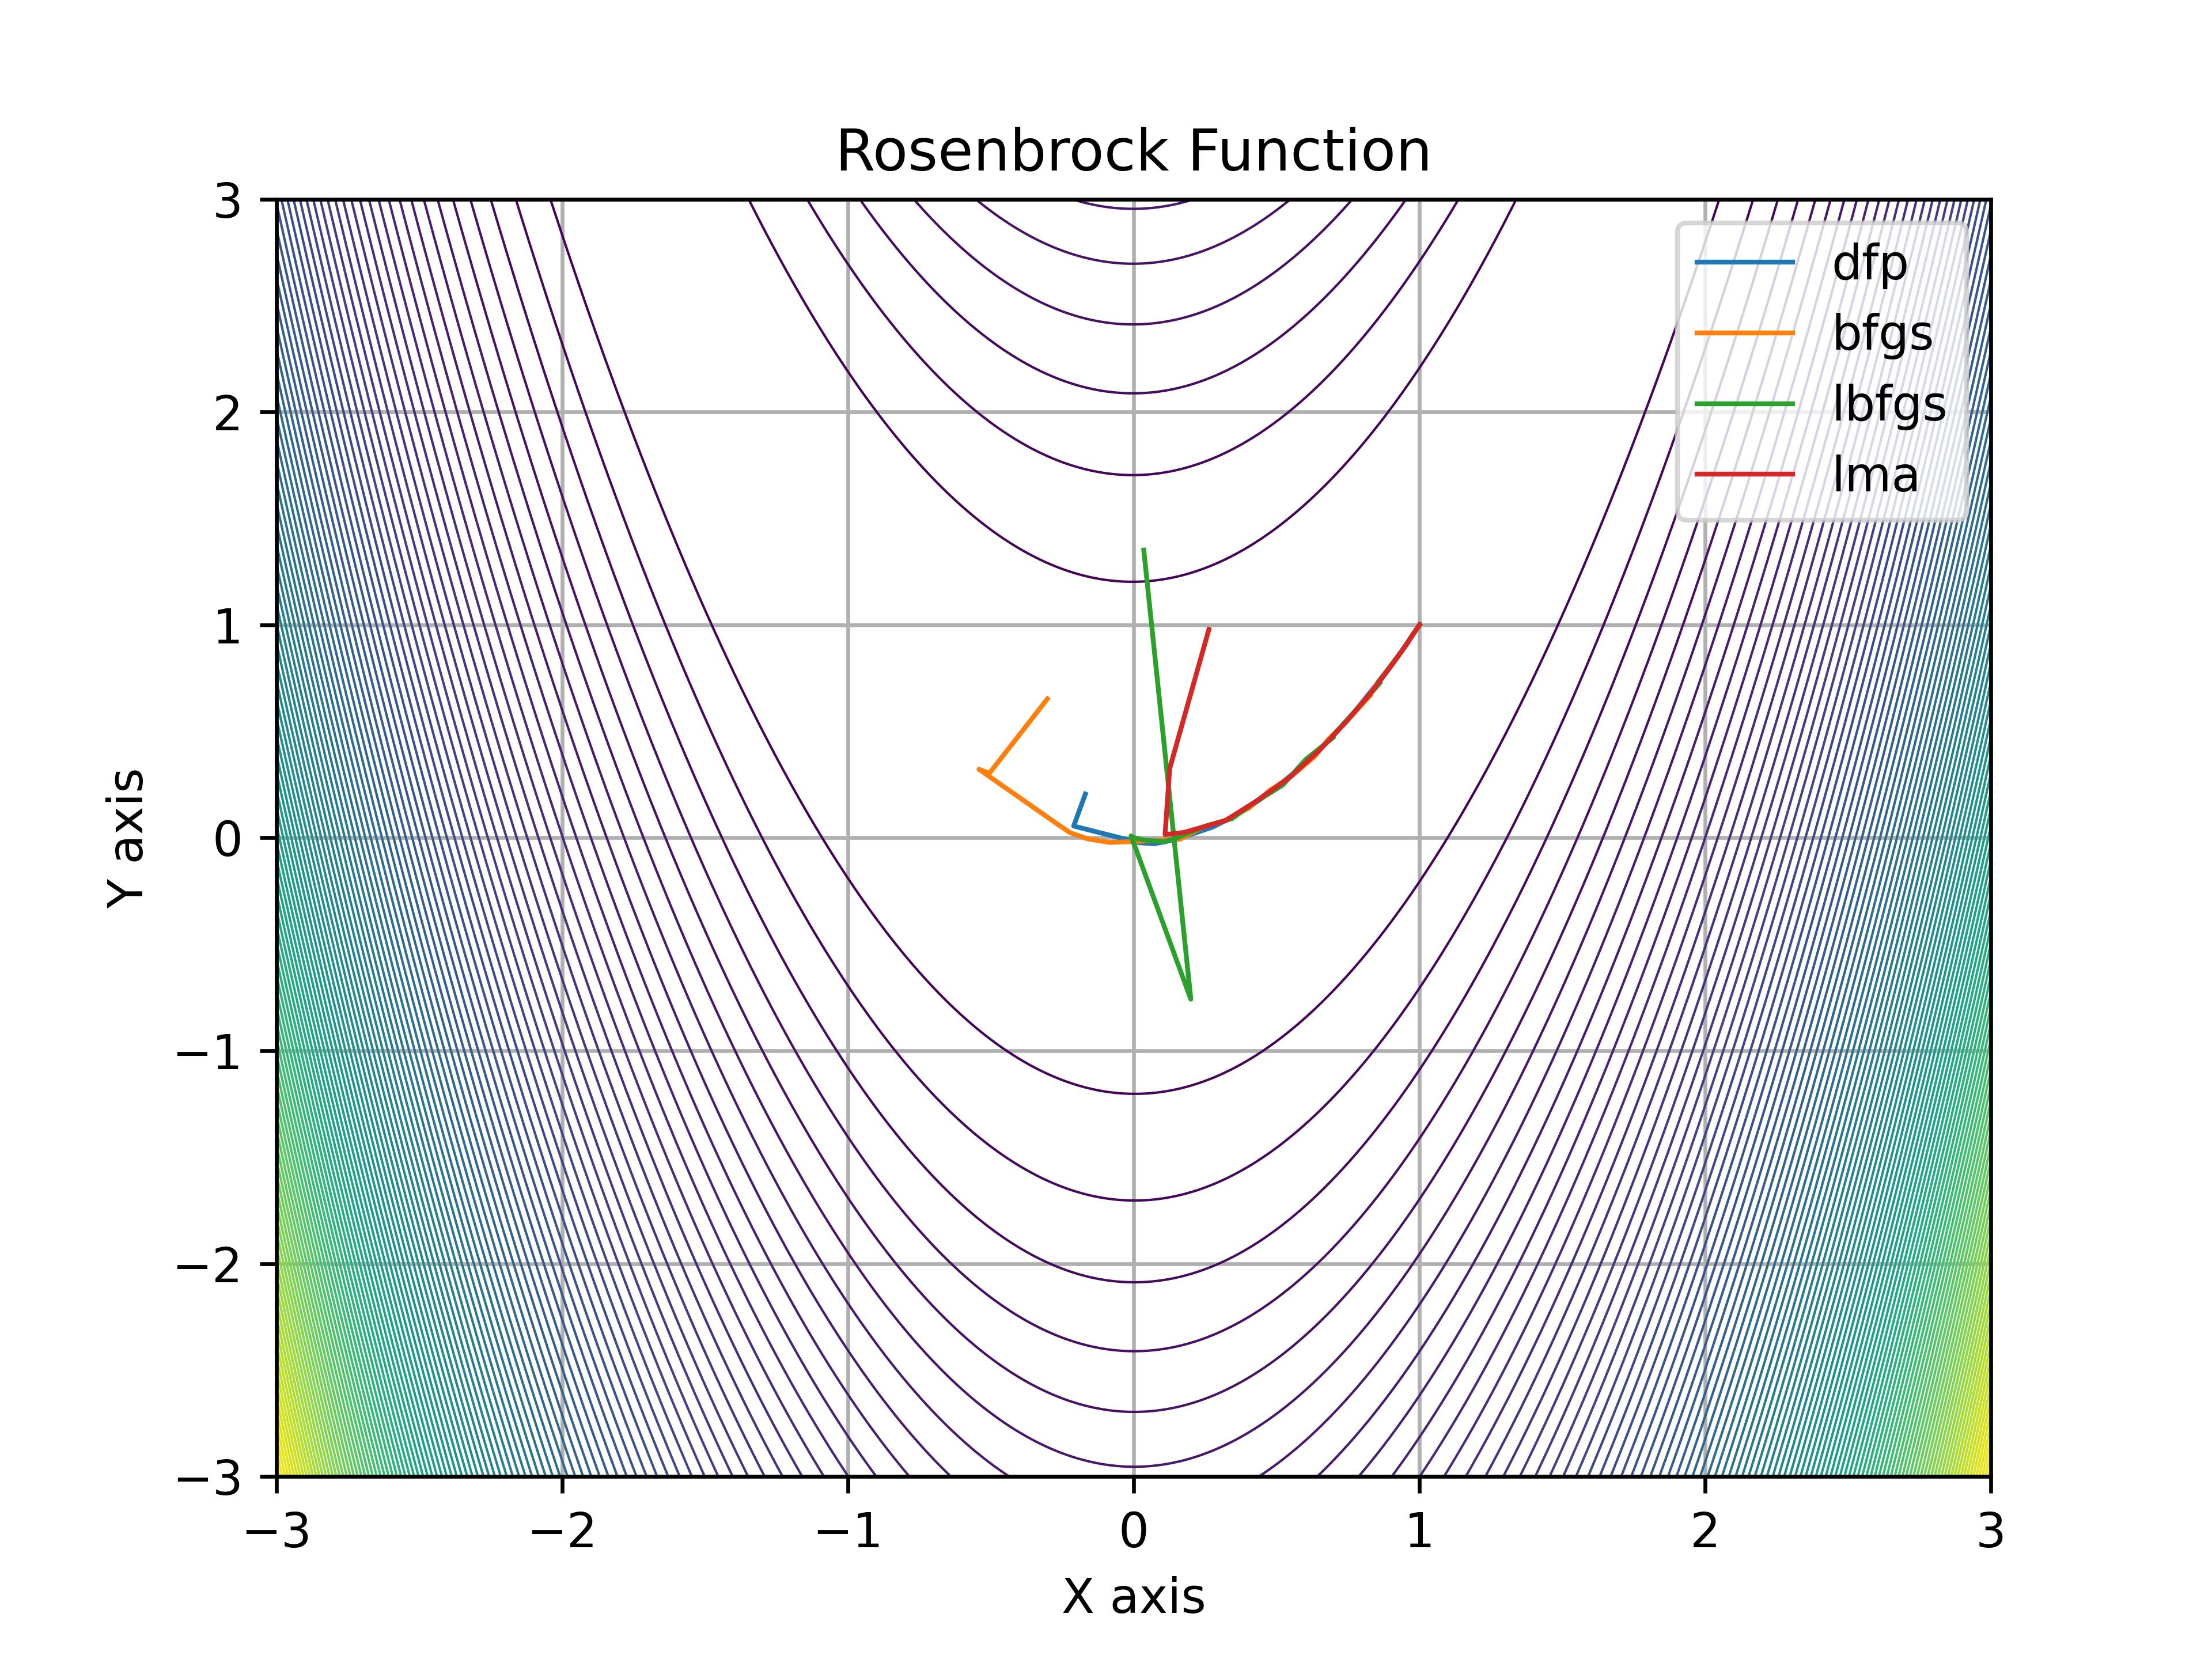
\includegraphics[scale=0.5]{images/rosenbrock2d.jpg}
\end{figure}
The isolines for Rosenbrock Function shows an interesting behaviour  near the optimal solution: the banana shape seems to force all algorithms to choose $x_{2}$ axis to solve first, and then solve for $x_{1}$ axis. The $x_{2}$ axis has probably the most significant derivative for an arbitrary point, so, when the algorithm walks around for solution, it first find the valley and then walks around the valley to find its minumum
\section{4D Function versions}
\label{functions4D}

\subsection{Rastrigin Function}
\label{rastrigin4d4D}

\subsubsection{Convergence Analysis}
\label{convergencerastrigin4d4D}


The convergence report for the Rastrigin Function in 4 dimensions is shown in Table~\ref{convergence:rastrigin4d}:

\begin{table}[H]
\centering
\caption{Convergence Report For Rastrigin Function}
\label{convergence:rastrigin4d}
\begin{tabular}{lrrrr}
\toprule
 Alg. &  Good &  Poor &  Diver. &  Total \\
\midrule
  dfp &   100 &     0 &       0 &    100 \\
 bfgs &   100 &     0 &       0 &    100 \\
lbfgs &   100 &     0 &       0 &    100 \\
  lma &   100 &     0 &       0 &    100 \\
\bottomrule
\end{tabular}
\end{table}

It is quite sure that all algorithms has good convergence for any algorithm for a
constrained search space of $\left[-0.15, 0.15\right]$. This search space is around
the optimal solution to avoid wrong convergence to a local minimum. In this search space,
Rastrigin Function has a well defined valley that has the solution as its center.
\subsubsection{Statistical Analysis of The Solutions}
\label{statisticalanalysisrastrigin4d4D}


The minimal. maximal, mean and median values of the solutions are shown in Table~\ref{function_values:rastrigin4d}:

\begin{table}[H]
\centering
\caption{Statistical Information about function values For Rastrigin Function}
\label{function_values:rastrigin4d}
\begin{tabular}{lrrrr}
\toprule
 Alg. &  Min &  Max &  Mean &  Median \\
\midrule
  dfp & 0.00 & 0.00 &  0.00 &    0.00 \\
 bfgs & 0.00 & 0.00 &  0.00 &    0.00 \\
lbfgs & 0.00 & 0.00 &  0.00 &    0.00 \\
  lma & 0.00 & 0.00 &  0.00 &    0.00 \\
\bottomrule
\end{tabular}
\end{table}

The values again are rounded. The median informs us that, for all
algorithms is expected to find the minimun of Rastrigin Function.
\subsubsection{Best Fits}
\label{bestfitsrastrigin4d4D}


The best solutions of all algorithms for Rastrigin Function, obtained using the minimal
distance of the solution, are shown in Table~\ref{solutions:rastrigin4d}:

\begin{table}[H]
\centering
\caption{Best Fits For Rastrigin Function}
\label{solutions:rastrigin4d}
\begin{tabular}{llrrr}
\toprule
 Alg. &    Sol. &  Iter. &  F. Eval &  F. Value \\
\midrule
  dfp & $S_{1}$ &     10 &       21 &      0.00 \\
 bfgs & $S_{2}$ &     11 &       61 &      0.00 \\
lbfgs & $S_{3}$ &      5 &      133 &      0.00 \\
  lma & $S_{4}$ &      4 &        5 &      0.00 \\
\bottomrule
\end{tabular}
\end{table}

LMA is the less expensive algorithm to solve Rastrigin in 4 dimensions, while LBFGS
is the most expensive of all. Although it has one more iteration than LMA, it evaluates
the objective function twice than BFGS, the second most expensive algorithm.

Although the column F. Value points to the the same value, this is a rounded value
and the real values are os order $10^{-22} \approx 10^{-14}$.


The best solutions of all algorithms for Rastrigin Function, indicated as
$S_{1}$, $S_{2}$, $S_{3}$ and $S_{4}$ in Table~\ref{solutions:rastrigin4d}, are shown
in Table~\ref{detailedsolutions:rastrigin4d}:

\begin{table}[H]
\centering
\caption{Detailed Solutions For Rastrigin Function}
\label{detailedsolutions:rastrigin4d}
\begin{tabular}{lrrrr}
\toprule
 Coord. &  $S_{1}$ &  $S_{2}$ &  $S_{3}$ &  $S_{4}$ \\
\midrule
$x_{1}$ &     0.00 &     0.00 &     0.00 &     0.00 \\
$x_{2}$ &    -0.00 &    -0.00 &     0.00 &     0.00 \\
$x_{3}$ &    -0.00 &    -0.00 &     0.00 &    -0.00 \\
$x_{4}$ &    -0.00 &    -0.00 &     0.00 &     0.00 \\
\bottomrule
\end{tabular}
\end{table}

The Table~\ref{detailedsolutions:rastrigin4d} shows the same solution to all algorithms, because the values are so small
and were rounded to fit on the Table. The differences of the optimal point are of order $10^{-14}$ to $10^{-22}$,
for the LMA, DFP, LBFGS and BFGS algorithms, respectively.

\subsection{Rosenbrock Function}
\label{rosenbrock4d4D}

\subsubsection{Convergence Analysis}
\label{convergencerosenbrock4d4D}


The convergence report for the Rosenbrock Function in 30 dimensions is shown in Table~\ref{convergence:rosenbrock4d}:

\begin{table}[H]
\centering
\caption{Convergence Report For Rosenbrock Function}
\label{convergence:rosenbrock4d}
\begin{tabular}{lrrrr}
\toprule
 Alg. &  Good &  Poor &  Diver. &  Total \\
\midrule
  dfp &    46 &    54 &       0 &    100 \\
 bfgs &    90 &    10 &       0 &    100 \\
lbfgs &    89 &    11 &       0 &    100 \\
  lma &    91 &     9 &       0 &    100 \\
\bottomrule
\end{tabular}
\end{table}

DFP has poor convergence properties for the Rosenbrock Function with more than 2 dimensions.
The rest have quite the same profile regarding convergence. It is important to note that
although all algorithms does not converge for the presented initial solutions, it does not
diverge at all. Because of the stop criterion of all algorithms, which is the function gradient value,
and the banana shaped valley (plateau) that Rosenbrock function has, we have this behaviour.
\subsubsection{Statistical Analysis of The Solutions}
\label{statisticalanalysisrosenbrock4d4D}


The minimal. maximal, mean and median values of the solutions are shown in Table~\ref{function_values:rosenbrock4d}:

\begin{table}[H]
\centering
\caption{Statistical Information about function values For Rosenbrock Function}
\label{function_values:rosenbrock4d}
\begin{tabular}{lrrrr}
\toprule
 Alg. &  Min &  Max &  Mean &  Median \\
\midrule
  dfp & 0.00 & 3.71 &  0.60 &    0.00 \\
 bfgs & 0.00 & 3.70 &  0.37 &    0.00 \\
lbfgs & 0.00 & 3.70 &  0.41 &    0.00 \\
  lma & 0.00 & 3.70 &  0.33 &    0.00 \\
\bottomrule
\end{tabular}
\end{table}


The median value informs us that all algorithms are like to find the solution
for Rosenbrock Function in 4 dimesions. The cases of poor convergence that all algorithms
have are reflected in the mean value. Looking at the Maximum value, it is noted that the mean value is
quite the same percentage shown in Table~\ref{convergence:rosenbrock4d}.

\subsubsection{Best Fits}
\label{bestfitsrosenbrock4d4D}


The best solutions of all algorithms for Rosenbrock Function, obtained using the minimal
distance of the solution, are shown in Table~\ref{solutions:rosenbrock4d}:

\begin{table}[H]
\centering
\caption{Best Fits For Rosenbrock Function}
\label{solutions:rosenbrock4d}
\begin{tabular}{llrrr}
\toprule
 Alg. &    Sol. &  Iter. &  F. Eval &  F. Value \\
\midrule
  dfp & $S_{1}$ &     44 &       49 &      0.00 \\
 bfgs & $S_{2}$ &     29 &       35 &      0.00 \\
lbfgs & $S_{3}$ &     45 &      134 &      0.00 \\
  lma & $S_{4}$ &     18 &       20 &      0.00 \\
\bottomrule
\end{tabular}
\end{table}

LMA is the less expensive algorithm to solve Rosenbrock Function in 4 dimensions, while LBFGS
is the most expensive of all. Although it has comparable iterations with DFP nd BFGS, it evaluates
the objective function twice as much of BFGS, the second most expensive algorithm.

Although the column F. Value points to the the same value, this is a rounded value
and the real values are os order $10^{-22} \approx 10^{-14}$.


The best solutions of all algorithms for Rosenbrock Function, indicated as
$S_{1}$, $S_{2}$, $S_{3}$ and $S_{4}$ in Table~\ref{solutions:rosenbrock4d}, are shown
in Table~\ref{detailedsolutions:rosenbrock4d}:

\begin{table}[H]
\centering
\caption{Detailed Solutions For Rosenbrock Function}
\label{detailedsolutions:rosenbrock4d}
\begin{tabular}{lrrrr}
\toprule
 Coord. &  $S_{1}$ &  $S_{2}$ &  $S_{3}$ &  $S_{4}$ \\
\midrule
$x_{1}$ &     1.00 &     1.00 &     1.00 &     1.00 \\
$x_{2}$ &     1.00 &     1.00 &     1.00 &     1.00 \\
$x_{3}$ &     1.00 &     1.00 &     1.00 &     1.00 \\
$x_{4}$ &     1.00 &     1.00 &     1.00 &     1.00 \\
\bottomrule
\end{tabular}
\end{table}

The optimal point of Rosenbrock function in 4 dimensions is correctly pointed to $\left[1, 1, 1, 1\right]$. The Table~\ref{detailedsolutions:rosenbrock4d}
shows the same solution to all algorithms, because the values are so small and were rounded to fit on the Table. The differences of
the optimal point are of order $10^{-14}$ to $10^{-22}$, for the LMA, DFP, LBFGS and BFGS algorithms, respectively.

\section{30D Function versions}
\label{functions30D}

\subsection{Rastrigin Function}
\label{rastrigin30d30D}

\subsubsection{Convergence Analysis}
\label{convergencerastrigin30d30D}


The convergence report for the Rastrigin Function in 2 dimensions is shown in Table~\ref{convergence:rastrigin30d}:

\begin{table}[H]
\centering
\caption{Convergence Report For Rastrigin Function}
\label{convergence:rastrigin30d}
\begin{tabular}{lrrrr}
\toprule
 Alg. &  Good &  Poor &  Diver. &  Total \\
\midrule
  dfp &   100 &     0 &       0 &    100 \\
 bfgs &   100 &     0 &       0 &    100 \\
lbfgs &   100 &     0 &       0 &    100 \\
  lma &   100 &     0 &       0 &    100 \\
\bottomrule
\end{tabular}
\end{table}


It is quite sure that all algorithms has good convergence for a
constrained search space of $\left[-0.15, 0.15\right]$. This search space is around
the optimal solution to avoid wrong convergence to a local minimum. In this search space,
Rastrigin Function has a well defined valley that has the solution as its center.
\subsubsection{Statistical Analysis of The Solutions}
\label{statisticalanalysisrastrigin30d30D}


The minimal. maximal, mean and median values of the solutions are shown in Table~\ref{function_values:rastrigin30d}:

\begin{table}[H]
\centering
\caption{Statistical Information about function values For Rastrigin Function}
\label{function_values:rastrigin30d}
\begin{tabular}{lrrrr}
\toprule
 Alg. &  Min &  Max &  Mean &  Median \\
\midrule
  dfp & 0.00 & 0.00 &  0.00 &    0.00 \\
 bfgs & 0.00 & 0.00 &  0.00 &    0.00 \\
lbfgs & 0.00 & 0.00 &  0.00 &    0.00 \\
  lma & 0.00 & 0.00 &  0.00 &    0.00 \\
\bottomrule
\end{tabular}
\end{table}

The values again are rounded. The median informs us that, for all
algorithms is expected to find the minimun of Rastrigin Function.
\subsubsection{Best Fits}
\label{bestfitsrastrigin30d30D}


The best solutions of all algorithms for Rastrigin Function, obtained using the minimal
distance of the solution, are shown in Table~\ref{solutions:rastrigin30d}:

\begin{table}[H]
\centering
\caption{Best Fits For Rastrigin Function}
\label{solutions:rastrigin30d}
\begin{tabular}{llrrr}
\toprule
 Alg. &    Sol. &  Iter. &  F. Eval &  F. Value \\
\midrule
  dfp & $S_{1}$ &      8 &       14 &      0.00 \\
 bfgs & $S_{2}$ &      9 &       54 &      0.00 \\
lbfgs & $S_{3}$ &      6 &      135 &      0.00 \\
  lma & $S_{4}$ &      4 &        5 &      0.00 \\
\bottomrule
\end{tabular}
\end{table}

LMA is the less expensive algorithm to solve Rastrigin in 30 dimensions, while LBFGS
is the most expensive of all. Although it has one more iteration than LMA, it evaluates
the objective function twice than BFGS, the second most expensive algorithm.

Although the column F. Value points to the the same value, this is a rounded value
and the real values are os order $10^{-22} \approx 10^{-14}$.


The best solutions of all algorithms for Rastrigin Function, indicated as
$S_{1}$, $S_{2}$, $S_{3}$ and $S_{4}$ in Table~\ref{solutions:rastrigin30d}, are shown
in Table~\ref{detailedsolutions:rastrigin30d}:

\begin{table}[H]
\centering
\caption{Detailed Solutions For Rastrigin Function}
\label{detailedsolutions:rastrigin30d}
\begin{tabular}{lrrrr}
\toprule
  Coord. &  $S_{1}$ &  $S_{2}$ &  $S_{3}$ &  $S_{4}$ \\
\midrule
 $x_{1}$ &    -0.00 &     0.00 &     0.00 &     0.00 \\
 $x_{2}$ &    -0.00 &     0.00 &     0.00 &     0.00 \\
 $x_{3}$ &    -0.00 &     0.00 &    -0.00 &    -0.00 \\
 $x_{4}$ &    -0.00 &     0.00 &     0.00 &     0.00 \\
 $x_{5}$ &     0.00 &    -0.00 &    -0.00 &    -0.00 \\
 $x_{6}$ &     0.00 &    -0.00 &    -0.00 &    -0.00 \\
 $x_{7}$ &     0.00 &    -0.00 &     0.00 &     0.00 \\
 $x_{8}$ &     0.00 &    -0.00 &    -0.00 &    -0.00 \\
 $x_{9}$ &    -0.00 &     0.00 &     0.00 &     0.00 \\
$x_{10}$ &    -0.00 &     0.00 &     0.00 &    -0.00 \\
$x_{11}$ &     0.00 &    -0.00 &     0.00 &     0.00 \\
$x_{12}$ &    -0.00 &     0.00 &     0.00 &     0.00 \\
$x_{13}$ &     0.00 &    -0.00 &    -0.00 &    -0.00 \\
$x_{14}$ &     0.00 &    -0.00 &     0.00 &     0.00 \\
$x_{15}$ &     0.00 &    -0.00 &    -0.00 &    -0.00 \\
$x_{16}$ &     0.00 &    -0.00 &    -0.00 &    -0.00 \\
$x_{17}$ &    -0.00 &     0.00 &    -0.00 &    -0.00 \\
$x_{18}$ &     0.00 &    -0.00 &    -0.00 &    -0.00 \\
$x_{19}$ &    -0.00 &     0.00 &    -0.00 &    -0.00 \\
$x_{20}$ &    -0.00 &     0.00 &    -0.00 &    -0.00 \\
$x_{21}$ &     0.00 &    -0.00 &     0.00 &     0.00 \\
$x_{22}$ &    -0.00 &     0.00 &    -0.00 &    -0.00 \\
$x_{23}$ &     0.00 &    -0.00 &    -0.00 &    -0.00 \\
$x_{24}$ &    -0.00 &     0.00 &    -0.00 &     0.00 \\
$x_{25}$ &    -0.00 &     0.00 &    -0.00 &     0.00 \\
$x_{26}$ &     0.00 &    -0.00 &     0.00 &     0.00 \\
$x_{27}$ &    -0.00 &     0.00 &     0.00 &     0.00 \\
$x_{28}$ &    -0.00 &     0.00 &    -0.00 &    -0.00 \\
$x_{29}$ &    -0.00 &     0.00 &    -0.00 &    -0.00 \\
$x_{30}$ &     0.00 &    -0.00 &    -0.00 &     0.00 \\
\bottomrule
\end{tabular}
\end{table}

The Table~\ref{detailedsolutions:rastrigin30d} shows the same solution to all algorithms, because the values are so small
and were rounded to fit on the Table. The differences of the optimal point are of order $10^{-14}$ to $10^{-22}$,
for the LMA, DFP, LBFGS and BFGS algorithms, respectively.


\subsection{Rosenbrock Function}
\label{rosenbrock30d30D}

\subsubsection{Convergence Analysis}
\label{convergencerosenbrock30d30D}


The convergence report for the Rosenbrock Function in 30 dimensions is shown in Table~\ref{convergence:rosenbrock30d}:

\begin{table}[H]
\centering
\caption{Convergence Report For Rosenbrock Function}
\label{convergence:rosenbrock30d}
\begin{tabular}{lrrrr}
\toprule
 Alg. &  Good &  Poor &  Diver. &  Total \\
\midrule
  dfp &     1 &    99 &       0 &    100 \\
 bfgs &    80 &    20 &       0 &    100 \\
lbfgs &    95 &     5 &       0 &    100 \\
  lma &    88 &    12 &       0 &    100 \\
\bottomrule
\end{tabular}
\end{table}

DFP has poor convergence properties for the Rosenbrock Function with more than 2 dimensions.
The rest have quite the same profile regarding convergence. It is important to note that
although all algorithms does not converge for the presented initial solutions, it does not
diverge at all. Because of the stop criterion of all algorithms, which is the function gradient value,
and the banana shaped valley (plateau) that Rosenbrock function has, we have this behaviour.
\subsubsection{Statistical Analysis of The Solutions}
\label{statisticalanalysisrosenbrock30d30D}


The minimal. maximal, mean and median values of the solutions are shown in Table~\ref{function_values:rosenbrock30d}:

\begin{table}[H]
\centering
\caption{Statistical Information about function values For Rosenbrock Function}
\label{function_values:rosenbrock30d}
\begin{tabular}{lrrrr}
\toprule
 Alg. &  Min &   Max &  Mean &  Median \\
\midrule
  dfp & 0.00 & 29.25 & 13.10 &   12.58 \\
 bfgs & 0.00 &  3.99 &  0.80 &    0.00 \\
lbfgs & 0.00 &  3.99 &  0.20 &    0.00 \\
  lma & 0.00 &  3.99 &  0.48 &    0.00 \\
\bottomrule
\end{tabular}
\end{table}

The median value informs us that all algorithms are like to find the solution
for Rosenbrock Function in 4 dimesions. The cases of poor convergence that all algorithms
have are reflected in the mean value. Looking at the Maximum value, it is noted that the mean value is
quite the same percentage shown in Table~\ref{convergence:rosenbrock30d}.

\subsubsection{Best Fits}
\label{bestfitsrosenbrock30d30D}

T
he best solutions of all algorithms for Rosenbrock Function, obtained using the minimal
distance of the solution, are shown in Table~\ref{solutions:rosenbrock4d}:

\begin{table}[H]
\centering
\caption{Best Fits For Rosenbrock Function}
\label{solutions:rosenbrock30d}
\begin{tabular}{llrrr}
\toprule
 Alg. &    Sol. &  Iter. &  F. Eval &  F. Value \\
\midrule
  dfp & $S_{1}$ &   2967 &     2990 &      0.00 \\
 bfgs & $S_{2}$ &    236 &      252 &      0.00 \\
lbfgs & $S_{3}$ &    164 &      406 &      0.00 \\
  lma & $S_{4}$ &     53 &      131 &      0.00 \\
\bottomrule
\end{tabular}
\end{table}

LMA is the less expensive algorithm to solve Rosenbrock Function in 30 dimensions, while DFP
is the most expensive of all.

Although the column F. Value points to the the same value, this is a rounded value
and the real values are os order $10^{-22} \approx 10^{-14}$.

The best solutions of all algorithms for Rosenbrock Function, indicated as
$S_{1}$, $S_{2}$, $S_{3}$ and $S_{4}$ in Table~\ref{solutions:rosenbrock30d}, are shown
in Table~\ref{detailedsolutions:rosenbrock30d}:

\begin{table}[H]
\centering
\caption{Detailed Solutions For Rosenbrock Function}
\label{detailedsolutions:rosenbrock30d}
\begin{tabular}{lrrrr}
\toprule
  Coord. &  $S_{1}$ &  $S_{2}$ &  $S_{3}$ &  $S_{4}$ \\
\midrule
 $x_{1}$ &     1.00 &     1.00 &     1.00 &     1.00 \\
 $x_{2}$ &     1.00 &     1.00 &     1.00 &     1.00 \\
 $x_{3}$ &     1.00 &     1.00 &     1.00 &     1.00 \\
 $x_{4}$ &     1.00 &     1.00 &     1.00 &     1.00 \\
 $x_{5}$ &     1.00 &     1.00 &     1.00 &     1.00 \\
 $x_{6}$ &     1.00 &     1.00 &     1.00 &     1.00 \\
 $x_{7}$ &     1.00 &     1.00 &     1.00 &     1.00 \\
 $x_{8}$ &     1.00 &     1.00 &     1.00 &     1.00 \\
 $x_{9}$ &     1.00 &     1.00 &     1.00 &     1.00 \\
$x_{10}$ &     1.00 &     1.00 &     1.00 &     1.00 \\
$x_{11}$ &     1.00 &     1.00 &     1.00 &     1.00 \\
$x_{12}$ &     1.00 &     1.00 &     1.00 &     1.00 \\
$x_{13}$ &     1.00 &     1.00 &     1.00 &     1.00 \\
$x_{14}$ &     1.00 &     1.00 &     1.00 &     1.00 \\
$x_{15}$ &     1.00 &     1.00 &     1.00 &     1.00 \\
$x_{16}$ &     1.00 &     1.00 &     1.00 &     1.00 \\
$x_{17}$ &     1.00 &     1.00 &     1.00 &     1.00 \\
$x_{18}$ &     1.00 &     1.00 &     1.00 &     1.00 \\
$x_{19}$ &     1.00 &     1.00 &     1.00 &     1.00 \\
$x_{20}$ &     1.00 &     1.00 &     1.00 &     1.00 \\
$x_{21}$ &     1.00 &     1.00 &     1.00 &     1.00 \\
$x_{22}$ &     1.00 &     1.00 &     1.00 &     1.00 \\
$x_{23}$ &     1.00 &     1.00 &     1.00 &     1.00 \\
$x_{24}$ &     1.00 &     1.00 &     1.00 &     1.00 \\
$x_{25}$ &     1.00 &     1.00 &     1.00 &     1.00 \\
$x_{26}$ &     1.00 &     1.00 &     1.00 &     1.00 \\
$x_{27}$ &     1.00 &     1.00 &     1.00 &     1.00 \\
$x_{28}$ &     1.00 &     1.00 &     1.00 &     1.00 \\
$x_{29}$ &     1.00 &     1.00 &     1.00 &     1.00 \\
$x_{30}$ &     1.00 &     1.00 &     1.00 &     1.00 \\
\bottomrule
\end{tabular}
\end{table}

The optimal point of Rosenbrock function in 30 dimensions is correctly pointed to $\left[1, 1, \cdots , 1, 1\right]$. The Table~\ref{detailedsolutions:rosenbrock30d}
shows the same solution to all algorithms, because the values are so small and were rounded to fit on the Table. The differences of
the optimal point are of order $10^{-14}$ to $10^{-22}$, for the LMA, DFP, LBFGS and BFGS algorithms, respectively.


\section{Discussion}

The main objective of this work is demonstrate the inner work of a optimization class of algorithms called \textit{Quasi-Newton algorithms}. Four of them are presented, along with the results and analysis regarding convergence, function evaluations and function objective values.

For implementation, it was decided to put constraints on search space, because for the original search space of some functions, like Ackley and Rastrigin, there are other minimas that will confuse every algorithm tested for this paper, and there is no sense on test a local minima procedure on these conditions. To restrain the initial solution to some region in the search space was a cheap and ready solution to avoid the algorithms to stop because of stumbling upon the wrong minimum.


The \textit{Levenberg-Marquardt Algorithm} implemented for this paper is very sensitive to hyperparameters, namely $\alpha$ and $\lambda$, which was not tunned to every function, so, the conspicuous performance variation is noticeable along the results. LMA is known to be fast and reliable, but in our implementation it was found a little tricky to get the hyperparameters right for all the test functions. But for Rosenbrock and Rastrigin, it is the best option, even for lame implementations like ours.

The \textit{Broyden–Fletcher–Goldfarb–Shanno} Algorithm was the only one that we decided to use it as is from \textit{SciPy}, because it has features desired for this work, like counting of function evaluations, gradient evaluation and iterations. It performed very well for Ackley and Booth Functions, and reasonably well for other functions.

The \textit{Davidon–Fletcher–Powell} Algorithm is not implemented in \textit{SciPy} but its equations shows that it is the dual of BFGS, so, it was easy to implement using some \textit{SciPy} code for BFGS algorithm. In the DFP procedure, there is a Hessian inversion to be evaluated every iteration, then, numerical imprecision would be taken into consideration evaluating its results. While in some cases it has a superb performance (Like Ackley Function), it has very poor performance in Rosenbrock Function and even in Beale Function. The increase of dimensions makes DFP suffer of numerical imprecision due to the Hessian inversion, except for Rastrigin, and it is the loser algorithm in other functions.

Finally, the \textit{Limited memory BFGS} has an average performance among the functions. The original algorithm was implemented using code found in the url https://github.com/qkolj/L-BFGS/blob/master/L-BFGS.ipynb.

In fact, there are no Quasi-Newton algorithms that solver the minima problem for an any function. From the standpoint of performance and convergence, all the algorithms have an average performance and a reasonable convergence, although we have to restrain the search space to a small area near the optimal solution.

\end{document}